%%%%%%%%%%%%%%%%%%%%%%%%%%%%%%%%%%%%%%%%%%%%%%%%%%%%%%%%%%%%%%%%%%%%%%%%%%%%%%
%  VISTA — Value-Informed Sequential Test-time Allocation
%  Elsevier CAS single-column (cas-sc), single-anonymous review
%
%  Overleaf: open via "CAS SC" template so cas-sc.cls is available.
%  Compile: pdflatex -> bibtex -> pdflatex -> pdflatex
%
%  NOTE: every \TODO{...} must be filled before submission.
%        Comment out \DRAFTMODE to hide all TODOs (dangerous).
%%%%%%%%%%%%%%%%%%%%%%%%%%%%%%%%%%%%%%%%%%%%%%%%%%%%%%%%%%%%%%%%%%%%%%%%%%%%%%

\documentclass[a4paper,fleqn]{cas-sc}

\usepackage[numbers,sort&compress]{natbib}
\usepackage{amsmath}
\usepackage{amssymb}
\usepackage{amsthm}                          % proposition, theorem, definition, remark
\DeclareMathOperator*{\argmax}{arg\,max}
\usepackage{booktabs}
\usepackage{needspace}
\usepackage{graphicx}
\usepackage{algorithm}
\usepackage{algpseudocode}
\usepackage{multirow}
\usepackage{placeins}
\usepackage{float}
\usepackage{caption}
\usepackage{threeparttable}
\usepackage{tcolorbox}
\usepackage{xspace}
\usepackage{xcolor}                          % \TODO color markers

\makeatletter
\def\fps@figure{htbp}
\makeatother

%% -----------------------------------------------------------------------
%% TODO marker — comment out \DRAFTMODE line before submission
%% -----------------------------------------------------------------------
%\newcommand{\DRAFTMODE}{}  % commented out for submission
\ifdefined\DRAFTMODE
  \newcommand{\TODO}[1]{{\color{red}\textbf{[TODO: #1]}}}
\else
  \newcommand{\TODO}[1]{#1}
\fi

%% -----------------------------------------------------------------------
%% Notation macros
%% -----------------------------------------------------------------------
\newcommand{\Hist}{\mathcal{H}}
\newcommand{\budget}{b}
\newcommand{\Bmax}{B_{\max}}
\newcommand{\Brier}{S}
\newcommand{\cost}{C}
\newcommand{\lossfn}{L}
\newcommand{\margval}{V}
\newcommand{\Exp}{\mathbb{E}}
\newcommand{\Prob}{\mathbb{P}}
\newcommand{\Ind}{\mathbf{1}}
\newcommand{\Real}{\mathbb{R}}

%% -----------------------------------------------------------------------
%% Theorem environments (amsthm)
%% -----------------------------------------------------------------------
\theoremstyle{plain}
\newtheorem{proposition}{Proposition}
\newtheorem{theorem}{Theorem}
\newtheorem{observation}{Observation}

\theoremstyle{definition}
\newtheorem{definition}{Definition}
\newtheorem{assumption}{Assumption}

\theoremstyle{remark}
\newtheorem*{remark}{Remark}

%%%%%%%%%%%%%%%%%%%%%%%%%%%%%%%%%%%%%%%%%%%%%%%%%%%%%%%%%%%%%%%%%%%%%%%%%%%%%%
\begin{document}
%%%%%%%%%%%%%%%%%%%%%%%%%%%%%%%%%%%%%%%%%%%%%%%%%%%%%%%%%%%%%%%%%%%%%%%%%%%%%%

\let\WriteBookmarks\relax
\def\floatpagefraction{0.7}
\def\textfraction{0.07}
\renewcommand{\topfraction}{0.9}
\renewcommand{\bottomfraction}{0.8}

\shorttitle{VISTA}
\shortauthors{Kong and Ha}

\title[mode=title]{VISTA: Value-Informed Sequential Test-time Allocation}

\author[1]{Jun-young Kong}
\ead{kong3162@konkuk.ac.kr}

\author[1]{Young-guk Ha\cormark[1]}
\ead{ygha@konkuk.ac.kr}

\affiliation[1]{organization={Department of Computer Science and Engineering, Konkuk University},
  addressline={120 Neungdong-ro, Gwangjin-gu},
  city={Seoul},
  postcode={05029},
  country={Republic of Korea}}

\cortext[1]{Corresponding author.}

%% -----------------------------------------------------------------------
%% Abstract
%% -----------------------------------------------------------------------
\begin{abstract}
We present \textbf{VISTA} (Value-Informed Sequential Test-time Allocation),
a prequential procedure for selecting reasoning budgets from deployment data
without a held-out calibration set.
VISTA combines randomized full-trajectory audits (fraction $\rho$ of queries)
to recover censored counterfactuals, importance-weighted policy comparison to
correct selection bias, and anytime-valid confidence sequences to prevent
spurious switching under continuous monitoring.
The need for these corrections is acute: omitting inverse-probability weighting
reverses policy rankings in five of eight experimental cells (wrong-best rate
$1.00$ in those cells), because early stopping censors the outcomes that longer
budgets would have produced.
A corpus audit across eight cells (two 8B reasoning models, four QA benchmarks)
documents qualitatively heterogeneous budget-response curves:
on MMLU-Pro accuracy is near-linear across the full token grid while the
hindsight per-item oracle reduces mean Brier by $30.1\%$;
on ARC-Challenge Brier saturates after the first budget step;
on MedMCQA and MedQA-USMLE one model's Brier worsens at nearly every budget
step while the other's improves---ruling out a universal fixed allocation.
VISTA at $\lambda{=}0$ (pure quality preservation) correctly stays at the
best fixed budget in all cells with adaptive headroom, achieving $\approx 0\%$ net
saving; this is the expected and intended behaviour of an error-controlled
procedure when no cheaper policy is certifiably better.
Increasing $\lambda$ controls the quality--compute exchange rate explicitly:
at $\lambda{=}0.01$, deployed VISTA achieves $3$--$35\%$ net token savings
with Brier increases $\leq 0.012$; at $\lambda{=}0.1$, savings reach
$9$--$59\%$ with Brier increases $\leq 0.019$---all with 95\% CIs from
200 stream-order permutations.
Confidence-threshold stopping, by contrast, increases Brier above the best
fixed budget in all eight cells ($+0.047$ to $+0.218$) while providing no
quality guarantees.
\end{abstract}

%% -----------------------------------------------------------------------
%% Highlights (3–5 items, max ~85 characters each)
%% -----------------------------------------------------------------------
\begin{highlights}
\item VISTA saves $3$--$59\%$ tokens with $\leq\!0.019$ Brier loss; no held-out set required.

\item Anytime-valid monitoring: zero false switches; greedy reaches $58.5\%$ FPR.

\item Unweighted comparison reverses policy rankings in 5 of 8 cells.

\item Budget-response curves differ across tasks and models; no universal fixed allocation.
\end{highlights}

%% -----------------------------------------------------------------------
%% Keywords
%% -----------------------------------------------------------------------
\begin{keywords}
Test-Time Compute \sep
Reasoning Language Models \sep
Adaptive Computation \sep
Calibration \sep
Sequential Decision Making \sep
Anytime-Valid Inference
\end{keywords}

\maketitle

%%%%%%%%%%%%%%%%%%%%%%%%%%%%%%%%%%%%%%%%%%%%%%%%%%%%%%%%%%%%%%%%%%%%%%%%%%%%%%
\section{Introduction}
\label{sec:introduction}
%%%%%%%%%%%%%%%%%%%%%%%%%%%%%%%%%%%%%%%%%%%%%%%%%%%%%%%%%%%%%%%%%%%%%%%%%%%%%%

Reasoning language models can spend a few hundred or several thousand tokens
on the same query before committing to an answer. Chain-of-thought prompting and
test-time inference strategies such as self-consistency, search, and repeated
sampling have established inference compute as an important axis of reasoning
performance~\cite{wei2022cot,kojima2022zeroshot,wang2023selfconsistency,yao2023tree,brown2024monkeys,snell2025scaling}.
More reasoning creates opportunities to correct mistakes, but it can also
consume compute without benefit or overturn an already correct answer
~\cite{chen2025overthinking,zhou2026overthinking}.
The practical deployment question is not \emph{whether} more reasoning helps
on average, but \emph{when} an additional block of reasoning is worth its cost
for the current query.

Two families of approaches address this question.
Fixed-budget policies run every query to the same token limit: simple and
predictable, but wasteful on easy queries and under-allocating on hard ones.
Heuristic early-exit methods stop when the model looks confident, using
trajectory signals such as maximum softmax probability, entropy, answer
stability, hidden-state probes, or convergence of intermediate predictions
~\cite{yang2026deer,wu2025thoughtcalibration,zhang2025selfverification,liu2025answerconvergence,sun2026refrain,xie2026statistical}.
Such signals can usefully indicate that reasoning has stabilised, yet empirical
self-evaluation and uncertainty studies show that confidence quality varies with
model, elicitation method, and domain~\cite{kadavath2022know,xiong2024uncertainty,kuhn2023semantic,zeng2025thinkingoutloud}. A stable prediction can therefore still be
wrong---and a wrong one can be corrected by further reasoning.

The core limitation of trajectory-only stopping is both empirical and
informational.
Empirically, we find that confidence-, entropy-, and stability-threshold
stopping \emph{increases} Brier above the best fixed budget in all eight
experimental cells ($+0.047$ to $+0.218$); signals trained on one model
fail to transfer to another on the same task.
The theoretical explanation is a non-identifiability result
(Observation~\ref{prop:impossibility}): for any estimator that is
simultaneously distribution-free, label-free at deployment time, and
restricted to a single unlabeled trajectory, the worst-case error in certifying
correctness is at least $\frac{1}{2}$.
Trajectory signals can be predictive under an empirical distribution without
constituting a distribution-free correctness certificate,
and their reliability does not transfer uniformly across model families
or task domains.

Rather than seeking a better correctness proxy, we change the decision target.
We ask whether an additional reasoning block improves a proper scoring loss
by more than its compute cost---the \emph{continuation value}---and learn the
answer from deployment outcomes once they become available.
Many workloads provide such delayed verifiable feedback naturally:
multiple-choice answers receive labels, programs are executed against tests,
and mathematical results are checked; verifier-based mathematical reasoning and
outcome-based supervision are representative examples~\cite{cobbe2021verifiers,uesato2022process}.
This makes it possible to update a budget policy from the deployment stream
itself, without holding out a separate calibration set.

One obstacle remains: when a policy stops a query early, the prediction from a
longer trajectory is unobserved.
We address this with randomized trajectory audits: a controlled fraction $\rho$
of arriving queries is continued to the maximum budget, revealing what each
candidate policy would have predicted.
Paired with delayed labels, these audits enable importance-weighted comparison
of multiple budget policies on the same items (Figure~\ref{fig:overview}).
The importance weight $1/\rho$ follows the classical inverse-probability
principle of Horvitz--Thompson estimation~\cite{horvitz1952sampling} and corrects
for the fact that audited items are observed under a known sampling mechanism;
omitting this correction reverses policy rankings in five of eight experimental
cells in our finite-sample replay experiments.

\begin{center}
  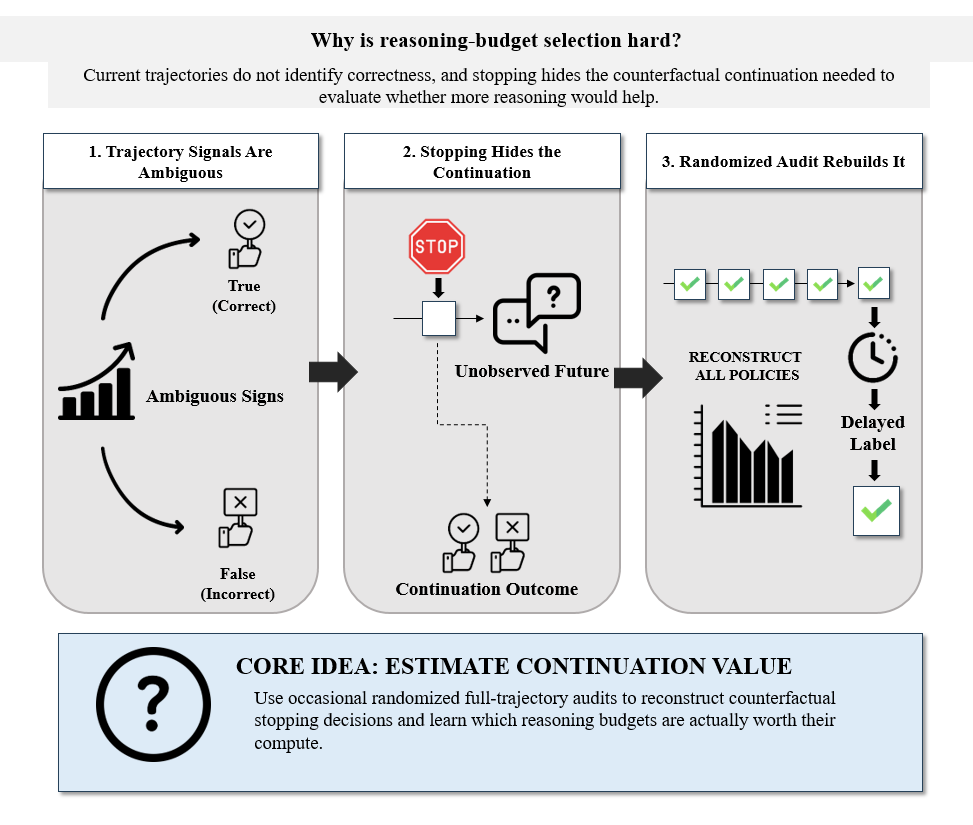
\includegraphics[width=\textwidth, height=0.55\textheight, keepaspectratio=true]{img1.png}
\end{center}
\begingroup
\captionof{figure}{Three interlocking obstacles in deployment-time
reasoning-budget selection and the VISTA response.
\textbf{(1)} Trajectory signals---confidence, answer stability,
entropy---are ambiguous: the same observable pattern is consistent with both
correct and incorrect predictions (Observation~\ref{prop:impossibility}).
\textbf{(2)} Stopping at budget $b$ hides the prediction that a longer
trajectory would have produced, blocking direct policy comparison from
deployment data alone.
\textbf{(3)} Randomized full-trajectory audits on a fraction $\rho$ of
items reconstruct the counterfactual, enabling importance-weighted comparison
of multiple budget policies once delayed labels arrive.}
\label{fig:overview}
\endgroup
\vspace{\baselineskip}

Estimates arrive sequentially and must be compared under continuous monitoring,
which creates additional risk: a procedure that switches to whichever policy
currently looks best acts on transient noise.
\textbf{VISTA} (Value-Informed Sequential Test-time Allocation) uses
anytime-valid confidence sequences---whose coverage guarantee holds at every
step, not just at a pre-specified sample size---to prevent spurious switches.
The prequential policy updates continuously as deployment outcomes arrive; all
audit compute is charged to the total cost so reported savings are real; no
model parameters are updated.

A corpus audit across four QA benchmarks and two 8B-parameter reasoning models
(Qwen3-8B~\cite{qwen3} and DeepSeek-R1-Distill-Llama-8B~\cite{deepseekr1}, both BF16) with a six-point
budget grid $\{256,\ldots,8192\}$ confirms that the marginal value of additional
reasoning is strongly task- and model-dependent.
Accuracy gains range from near-linear (MMLU-Pro, $47.7\%\to73.8\%$ across the
grid) to early-saturating (ARC-Challenge, most gain in the first budget step);
patterns invert across models on the same task.
The hindsight oracle reduces mean Brier by $30.1\%$ on MMLU-Pro, with
$76.1\%$ of items meeting a per-item quality threshold at a budget below the
maximum; a constrained matched-mean-quality oracle passes the adaptive-opportunity
test (Gate~0) in six of eight cells.
A fixed confidence gate increases Brier above the best fixed budget in all
eight cells, confirming that deployable item-adaptive allocation cannot rely
on naive stopping heuristics.

\paragraph{Contributions.}
\begin{enumerate}
\item \textbf{IPW necessity for unbiased policy-risk estimation.}
We show that omitting inverse-probability weighting reverses policy rankings
in 5 of 8 cells (wrong-best rate 1.00); IPW reduces bias $2.2\times$--$23\times$
and is a necessary, not optional, correction whenever early stopping censors
counterfactual trajectories.
\item \textbf{Continuation-value formulation.}
We replace the unobservable correctness target with the \emph{continuation value}---
expected improvement in proper scoring loss per additional token---estimable
from delayed deployment feedback without a held-out split.
\item \textbf{VISTA.}
A prequential budget-selection procedure combining randomized audits,
IPW policy comparison, and anytime-valid confidence sequences.
At $\lambda{=}0.01$--$0.1$, deployed VISTA achieves $3$--$59\%$ net token
savings with Brier increases ${\leq}0.019$ (95\% CIs, 200 permutations).
\item \textbf{Systematic empirical audit.}
Eight cells (two models, four QA benchmarks) documenting heterogeneous
budget-response curves, item-level allocation headroom, and per-component
ablation---including the finding that confidence-threshold stopping degrades
Brier in all eight cells.
\end{enumerate}

%%%%%%%%%%%%%%%%%%%%%%%%%%%%%%%%%%%%%%%%%%%%%%%%%%%%%%%%%%%%%%%%%%%%%%%%%%%%%%
\section{Related Work}
\label{sec:related}
%%%%%%%%%%%%%%%%%%%%%%%%%%%%%%%%%%%%%%%%%%%%%%%%%%%%%%%%%%%%%%%%%%%%%%%%%%%%%%

\paragraph{Test-time compute scaling and adaptive allocation.}
Chain-of-thought prompting established that explicitly generated intermediate
reasoning can improve language-model performance~\cite{wei2022cot,kojima2022zeroshot}.
Subsequent inference-time strategies scale compute through repeated reasoning
paths, self-consistency, search, or repeated sampling
~\cite{wang2023selfconsistency,yao2023tree,brown2024monkeys}.
Snell et al.~\cite{snell2025scaling} show that the effectiveness of test-time
compute depends strongly on prompt difficulty and motivate compute-optimal
allocation across instances. More recent work makes the allocation problem
explicit: Zhai et al.~\cite{zhai2026adaptive} solve a constrained
accuracy--compute problem and train a lightweight allocator to imitate oracle
actions. In parallel, analyses of long-reasoning models document diminishing
returns and overthinking, including unnecessary computation on easy problems
and reversals of previously correct answers
~\cite{chen2025overthinking,zhou2026overthinking}.
VISTA shares the premise that inference compute should be adaptive, but treats
the value of continuation as a deployment-time quantity learned sequentially
from delayed outcomes rather than as an offline oracle label or a fixed
instance-difficulty score.

\paragraph{Adaptive computation and early exit.}
Adaptive computation predates reasoning LLMs. Adaptive Computation Time and
PonderNet learn how much computation a neural network should spend on an input
~\cite{graves2016adaptive,banino2021pondernet}, while DeeBERT, FastBERT, and
confidence-based layer exiting reduce transformer inference by terminating easy
examples early~\cite{xin2020deebert,liu2020fastbert,schwartz2020righttool}.
Recent reasoning-specific methods move the stopping decision inside the
chain-of-thought trajectory. DEER uses confidence at trial-answer transition
points~\cite{yang2026deer}; Thought Calibration uses lightweight hidden-state
probes to detect when novel reasoning plateaus~\cite{wu2025thoughtcalibration};
Answer Convergence uses consistency of intermediate answers
~\cite{liu2025answerconvergence}; REFRAIN adapts stopping thresholds from
reflective redundancy~\cite{sun2026refrain}; and TERMINATOR learns optimal
exit positions from hindsight labels~\cite{nagle2026terminator}.
Other approaches reject low-value partial trajectories using reward signals
~\cite{cheshmi2025earlyrejection}, combine hidden-state probes with split
conformal control~\cite{akgul2025lynx}, or apply sequential uncertainty tests
directly during reasoning~\cite{xie2026statistical}.
These methods establish that trajectory signals can be useful for efficiency.
VISTA addresses a complementary question: after early stopping makes larger
budgets counterfactually unobserved, how can deployment feedback be used to
compare the realised risk of candidate budget policies on a common statistical
scale?

\paragraph{Self-evaluation, uncertainty, and calibration in language models.}
Modern neural networks can be miscalibrated even when classification accuracy is
high~\cite{guo2017calibration}. Language models nevertheless contain useful
self-evaluation signals: Kadavath et al.~\cite{kadavath2022know} show that
models can often predict whether they know an answer, while black-box confidence
elicitation~\cite{xiong2024uncertainty}, semantic uncertainty
~\cite{kuhn2023semantic}, and sampling-based consistency
~\cite{manakul2023selfcheckgpt} provide additional failure-prediction signals.
For reasoning models specifically, hidden-state probes can predict intermediate
answer correctness~\cite{zhang2025selfverification}, and verbalized confidence
changes with reasoning-model training and task conditions
~\cite{zeng2025thinkingoutloud}. These findings are compatible with
Observation~\ref{prop:impossibility}: a signal can be predictive under an
empirical distribution without constituting a distribution-free correctness
certificate. VISTA therefore treats confidence and related quantities as
candidate policy features rather than as ground-truth stopping criteria.

\paragraph{Proper scoring rules and probabilistic quality.}
Because additional reasoning can change the full predictive distribution even
when top-1 accuracy is unchanged, we evaluate continuation with proper scoring
rules. The Brier score originates with Brier~\cite{brier1950verification};
strict propriety and the general decision-theoretic role of scoring rules are
formalised by Gneiting and Raftery~\cite{gneiting2007strictly}; and the
reliability--resolution--uncertainty decomposition used in
Eq.~\eqref{eq:decomposition} follows Murphy~\cite{murphy1973new}.
This distinction matters in our setting because accuracy-, Brier-, and
log-loss-optimal reasoning budgets can disagree on the same model--dataset cell.

\paragraph{Distribution-free calibration and risk control.}
Conformal prediction provides distribution-free predictive guarantees under
exchangeability~\cite{vovk2005algorithmic,lei2018conformal}. Risk-controlling
prediction sets~\cite{bates2021rcps}, Learn-then-Test
~\cite{angelopoulos2025ltt}, and Conformal Risk Control
~\cite{angelopoulos2024crc} extend calibration from coverage to user-specified
losses. Conformal Language Modeling applies related ideas to generative models
by calibrating sampling and rejection rules~\cite{quach2024conformal}.
Most directly, Conformal Thinking formulates reasoning-budget selection as a
risk-control problem and calibrates upper and lower stopping thresholds from a
validation set~\cite{wang2026conformalthinking}; it is the closest in spirit to
VISTA and likely achieves stronger savings in settings where a held-out split is
available.
VISTA targets a different regime: no calibration split is reserved (labels
arrive sequentially after deployment decisions), and early stopping censors the
outcomes of longer budget policies.
Randomized trajectory audits are introduced specifically to recover those
missing counterfactual outcomes, and anytime-valid monitoring replaces the
static conformal guarantee with one that holds continuously as feedback arrives.
A direct empirical comparison would require adapting Conformal Thinking to
the streaming, censored-label setting, which we leave for future work.

\paragraph{Inverse-probability weighting and anytime-valid inference.}
VISTA combines two statistical ideas that solve different problems. First,
known audit probabilities permit Horvitz--Thompson inverse-probability
weighting~\cite{horvitz1952sampling}, which targets the population policy-risk
contrast despite randomized observation of full trajectories. Second, repeated
inspection of accumulating evidence requires time-uniform rather than
fixed-sample uncertainty quantification. Confidence sequences provide
nonasymptotic coverage uniformly over time~\cite{howard2021confidence};
betting-based constructions yield sharp confidence sequences for bounded means
~\cite{waudbysmith2024betting}; and e-processes provide a broader framework for
safe anytime-valid inference under optional stopping~\cite{ramdas2023safe}.
Thus IPW corrects \emph{which trajectories are observed}, whereas confidence
sequences control \emph{when policy comparisons are inspected and acted upon}.
Concurrent work by Yu et al.~\cite{yu2026bpac} (B-PAC) proposes an anytime-safe
PAC-efficient stopping rule for reasoning that also combines statistical
efficiency with online safety guarantees. B-PAC targets sample efficiency under
a fixed computational budget; VISTA targets deployment-stream budget selection
under counterfactual censoring from early stopping. The two frameworks share
the commitment to statistical safety guarantees but address different aspects
of the test-time compute allocation problem.

\paragraph{Positioning of VISTA.}
The closest contemporaneous approaches include confidence-based dynamic early
exit~\cite{yang2026deer}, hidden-state thought calibration
~\cite{wu2025thoughtcalibration}, answer-convergence stopping
~\cite{liu2025answerconvergence}, statistically monitored early stopping
~\cite{xie2026statistical}, conformal risk-controlled reasoning
~\cite{wang2026conformalthinking}, supervised adaptive compute allocation
~\cite{zhai2026adaptive}, and anytime-safe PAC-efficient reasoning
~\cite{yu2026bpac}. VISTA does not argue that these signals or controls
are ineffective. Its distinguishing layer is counterfactual policy evaluation
from a live deployment stream: occasional randomized continuations reveal the
otherwise missing larger-budget outcomes, delayed labels convert them into
policy losses, inverse-probability weighting corrects the observation scheme,
and anytime-valid inference governs repeated policy updates without a held-out
calibration split.

%%%%%%%%%%%%%%%%%%%%%%%%%%%%%%%%%%%%%%%%%%%%%%%%%%%%%%%%%%%%%%%%%%%%%%%%%%%%%%
\section{Preliminaries and a Non-identifiability Observation}
\label{sec:impossibility}
%%%%%%%%%%%%%%%%%%%%%%%%%%%%%%%%%%%%%%%%%%%%%%%%%%%%%%%%%%%%%%%%%%%%%%%%%%%%%%

Fix a query $x$ with ground-truth answer $y^{\star}$. A reasoning model
produces a trajectory $r_{1:\Bmax}$, and at each checkpoint $\budget$ we may
force termination and read off a candidate answer $\hat{y}_{\budget}$ together
with a predictive distribution $\hat{p}_{\budget} \in \Delta^{C-1}$. Write the
observable history as
\begin{equation}
  \Hist_{\budget} =
  \bigl(x,\;r_{1:\budget},\;\mathrm{logits}_{1:\budget},\;
  \hat{y}_{\budget},\;\hat{p}_{\budget}\bigr),
\end{equation}
and the unobserved correctness indicator as
$Y_{\budget} = \Ind\{\hat{y}_{\budget} = y^{\star}\}$.

\begin{observation}[Non-identifiability of label-free correctness]
\label{prop:impossibility}
Let $f$ be any measurable estimator
$\hat{a}_{\budget} = f(\Hist_{\budget})$.
There exist two joint distributions $\Prob_{0},\Prob_{1}$ over
$(\Hist_{\budget},Y_{\budget})$ with identical marginals on $\Hist_{\budget}$
such that $Y_{\budget}=0$ a.s.\ under $\Prob_{0}$ and $Y_{\budget}=1$
a.s.\ under $\Prob_{1}$. Consequently, for every $\Hist_{\budget}$,
\begin{equation}
  \max\Bigl\{|\hat{a}_{\budget}-0|,\;|\hat{a}_{\budget}-1|\Bigr\}
  \geq \tfrac{1}{2},
\end{equation}
and no non-trivial distribution-free finite-sample lower bound on
$\Prob(Y_{\budget}=1\mid\Hist_{\budget})$ exists.
\end{observation}

\begin{proof}
Given any $\Prob_0$ over $(\Hist_b, Y_b)$, construct $\Prob_1$ by relabelling
$y^\star$ to equal $\hat{y}_b$ on every realisation of $\Hist_b$.
Since $y^\star$ appears nowhere in $\Hist_b$, the marginal distribution
$\Prob_1(\Hist_b=h) = \Prob_0(\Hist_b=h)$ for every $h$, while
$Y_b = 1$ $\Prob_1$-a.s.\ and $Y_b = 0$ $\Prob_0$-a.s.

Any measurable estimator $f$ satisfies $f(\Hist_b) = \hat{a}_b \in \mathbb{R}$
deterministically given $\Hist_b$.
For any fixed realisation $h$, let $v = f(h)$.
Then $|\hat{a}_b - 0| = |v|$ under $\Prob_0$ and $|\hat{a}_b - 1| = |1-v|$
under $\Prob_1$.
Since $\max\{|v|, |1-v|\} \ge \tfrac{1}{2}$ for all $v \in \mathbb{R}$
(with equality iff $v = \tfrac{1}{2}$), the bound holds pointwise for every
realisation $h$ of $\Hist_b$, hence in expectation under both $\Prob_0$ and
$\Prob_1$.
The non-existence of a non-trivial distribution-free lower bound on
$\Prob(Y_b=1|\Hist_b)$ follows by the same coupling:
any lower bound $L(h) > 0$ fails under $\Prob_0$ (where $Y_b = 0$ a.s.),
and any lower bound $L(h) < 1$ fails under $\Prob_1$ (where $Y_b = 1$ a.s.).
\end{proof}

The obstruction is informational: collecting additional unlabelled trajectories
cannot remove it without assumptions connecting observable model behaviour to
ground-truth correctness. Self-consistency, answer stability, and related
trajectory-based quantities are descriptive signals but do not constitute
correctness guarantees.

\begin{remark}
Observation~\ref{prop:impossibility} is a standard label-free learning
result~\cite{shalev2014understanding}: any measurable function of the unlabeled
trajectory is a constant from the perspective of the label.
Its role here is to explain the empirical failure documented in
Section~\ref{sec:baselines}: threshold stopping degrades Brier in all eight
cells not because of poor threshold calibration but because trajectory signals
are, in the worst case, uninformative about correctness.
The result does \emph{not} assert that signals are useless under an empirical
distribution, nor that they cannot guide stopping heuristics in practice;
it asserts that no such method carries a distribution-free correctness
certificate. Methods that condition on a held-out calibration set (e.g.,
Conformal Thinking~\cite{wang2026conformalthinking}) or on labelled
supervision are explicitly outside this scope.
\end{remark}

%%%%%%%%%%%%%%%%%%%%%%%%%%%%%%%%%%%%%%%%%%%%%%%%%%%%%%%%%%%%%%%%%%%%%%%%%%%%%%
\section{Continuation Value and Budget Selection}
\label{sec:formulation}
%%%%%%%%%%%%%%%%%%%%%%%%%%%%%%%%%%%%%%%%%%%%%%%%%%%%%%%%%%%%%%%%%%%%%%%%%%%%%%

\subsection{Loss}

Let $\budget_1 < \cdots < \budget_K = \Bmax$ be a globally fixed budget grid.
For item $i$ at checkpoint $j$ we use the \emph{summed} multiclass Brier score
~\cite{brier1950verification,gneiting2007strictly}
\begin{equation}
  \Brier_{i,j}
  = \bigl\lVert\hat{p}_{i,j} - e_{y_i}\bigr\rVert_2^2
  = \sum_{c=1}^{C}\bigl(\hat{p}_{i,j,c} - \mathbf{1}_{c=y_i}\bigr)^2,
\end{equation}
where the sum over classes is not divided by $C$.  This is the standard
proper-scoring form; dividing by $C$ would yield a differently scaled variant
with different decomposition constants.
We define the deployment loss
\begin{equation}
  \lossfn^{(\lambda)}_{i,j} = \Brier_{i,j} + \lambda\,\cost_{i,j},
  \qquad \lambda\geq 0,
\end{equation}
where $\cost_{i,j} = b_j / \Bmax \in [0,1]$ is realised compute normalised
by the maximum budget so that $\lambda$ is on the same scale as the Brier
score; $\lambda$ is a user-specified quality--compute exchange rate reported
over a range of values rather than a single operating point.
At $\lambda{=}0.01$ the maximum cost penalty is $0.01$ Brier units;
at $\lambda{=}0.1$ it is $0.1$ Brier units.

\subsection{Marginal value and its decomposition}

\begin{definition}[Marginal value of a reasoning block]
The marginal value of continuing from checkpoint $j$ to $j+1$ is
\begin{equation}
  \margval_j(\lambda)
  =
  \Exp\!\left[\Brier_{i,j}-\Brier_{i,j+1}\right]
  -\lambda\,\Exp\!\left[\cost_{i,j+1}-\cost_{i,j}\right].
\end{equation}
\end{definition}

Applying the classical reliability--resolution--uncertainty decomposition
~\cite{murphy1973new},
$\Exp[\Brier_j] = \mathrm{REL}_j - \mathrm{RES}_j + \mathrm{UNC}$
and noting that UNC cancels across budgets yields
\begin{equation}
  \margval_j(\lambda)
  =
  \underbrace{\bigl(\mathrm{RES}_{j+1}-\mathrm{RES}_j\bigr)}_{\text{change in resolution}}
  -
  \underbrace{\bigl(\mathrm{REL}_{j+1}-\mathrm{REL}_j\bigr)}_{\text{change in reliability error}}
  -\lambda\,\Delta\cost_j.
  \label{eq:decomposition}
\end{equation}
Equation~\eqref{eq:decomposition} separates two ways an additional reasoning
block can change probabilistic quality. Whether further reasoning tends to
improve accuracy while degrading calibration, improve both, or degrade both is
an empirical question that may vary across models, datasets, and budget
intervals. We treat the sign and magnitude of each component as a measurable
outcome rather than a structural claim.

%%%%%%%%%%%%%%%%%%%%%%%%%%%%%%%%%%%%%%%%%%%%%%%%%%%%%%%%%%%%%%%%%%%%%%%%%%%%%%
\section{VISTA}
\label{sec:method}
%%%%%%%%%%%%%%%%%%%%%%%%%%%%%%%%%%%%%%%%%%%%%%%%%%%%%%%%%%%%%%%%%%%%%%%%%%%%%%

\subsection{Scope}

\begin{assumption}[Delayed verifiable feedback]
\label{asm:feedback}
For each item $i$, the outcome $y_i$ becomes available after a finite delay
through exact-answer matching, program execution, formal verification, or
post-hoc adjudication.
\end{assumption}

Tasks with open-ended generation and no eventual feedback lie outside this
setting. Automatically checked mathematical answers, executable programs, and
verifier-based reasoning provide representative sources of delayed outcome
feedback~\cite{cobbe2021verifiers,uesato2022process,brown2024monkeys}.

\subsection{Randomized full-trajectory audits}

To observe counterfactual predictions at larger budgets, we randomly select
items for full-trajectory auditing:
\begin{equation}
  A_i \sim \mathrm{Bernoulli}(\rho_i).
\end{equation}
Audited items ($A_i=1$) are run through $\Bmax$ and all checkpoint predictions
retained. For policy $\pi$ with stopping checkpoint $\tau_\pi(\Hist_i)$,
define the realised loss
\begin{equation}
  \ell_i(\pi) = \Brier_{i,\tau_\pi} + \lambda\,\cost_{i,\tau_\pi}.
\end{equation}
Following inverse-probability weighting for unequal observation probabilities
~\cite{horvitz1952sampling}, the importance-weighted comparison against a
reference policy $\pi_{\mathrm{ref}}$ is
\begin{equation}
  X_i(\pi)
  = \frac{A_i}{\rho_i}
    \bigl[\ell_i(\pi) - \ell_i(\pi_{\mathrm{ref}})\bigr],
  \label{eq:policy-ipw}
\end{equation}
with $\Exp[X_i(\pi)\mid\mathcal{F}_{i-1}] = R(\pi)-R(\pi_{\mathrm{ref}})$
where $R(\pi)=\Exp[\ell_i(\pi)]$. The audit probability $\rho_i$ may depend
on past observations, provided it is set before the current outcome is
revealed. All audit computation counts toward reported total compute.

\subsection{Anytime-valid policy evaluation}

We maintain simultaneous confidence sequences for the excess risk of every
policy relative to the reference~\cite{howard2021confidence,waudbysmith2024betting,ramdas2023safe}. For finite family $\Pi$, the guarantee is
\begin{equation}
  \Prob\!\Bigl(
    \forall n,\;\forall\pi\in\Pi:\;
    R(\pi)-R(\pi_{\mathrm{ref}})
    \in[\underline{\Delta}_{\pi,n},\,\overline{\Delta}_{\pi,n}]
  \Bigr) \geq 1-\alpha,
\end{equation}
constructed via bounded empirical-Bernstein sequences or betting-based methods
with simultaneous coverage across all policies.

\subsection{Policy family}

Candidate policies include fixed-budget rules, predictive-confidence
thresholds, entropy thresholds, answer-stability rules, top-1/top-2 margin
thresholds, and confidence-slope thresholds. A generic threshold policy is
\begin{equation}
  \tau_\theta(\Hist_i) = \min\{j : s_{i,j}\leq\theta_j\},
  \qquad \theta\in\Theta,\quad|\Theta|<\infty.
\end{equation}
Every audited trajectory permits reconstruction of the stopping checkpoint and
realised loss for every member of this finite family.

\begin{algorithm}[t]
\caption{VISTA: prequential reasoning-budget selection}
\label{alg:mvtcs}
\begin{algorithmic}[1]
\Require budget grid $\{\budget_j\}_{j=1}^{K}$, policy family $\Pi$,
         exchange rate $\lambda$, confidence level $\alpha$,
         audit schedule $\{\rho_i\}$
\State Initialise confidence sequences for all $\pi\in\Pi$
\For{each arriving item $i$}
  \State Select the currently preferred active policy $\pi_i$
  \State Execute reasoning process according to $\pi_i$
  \State Draw $A_i\sim\mathrm{Bernoulli}(\rho_i)$ before observing outcome
  \If{$A_i=1$}
    \State Continue item to $\Bmax$; retain all checkpoint predictions
  \EndIf
  \State Deploy the answer produced by $\pi_i$
  \State \textbf{When $y_i$ arrives:}
  \If{$A_i=1$}
    \State Reconstruct $\ell_i(\pi)$ for all $\pi\in\Pi$ from checkpoint predictions
    \State Form importance-weighted risk differences via Eq.~\eqref{eq:policy-ipw}
    \State Update confidence sequences for all $\pi\in\Pi$
    \State Identify currently preferred policy $\pi_{i+1}$ from updated sequences
  \EndIf
\EndFor
\end{algorithmic}
\end{algorithm}

\begin{center}
  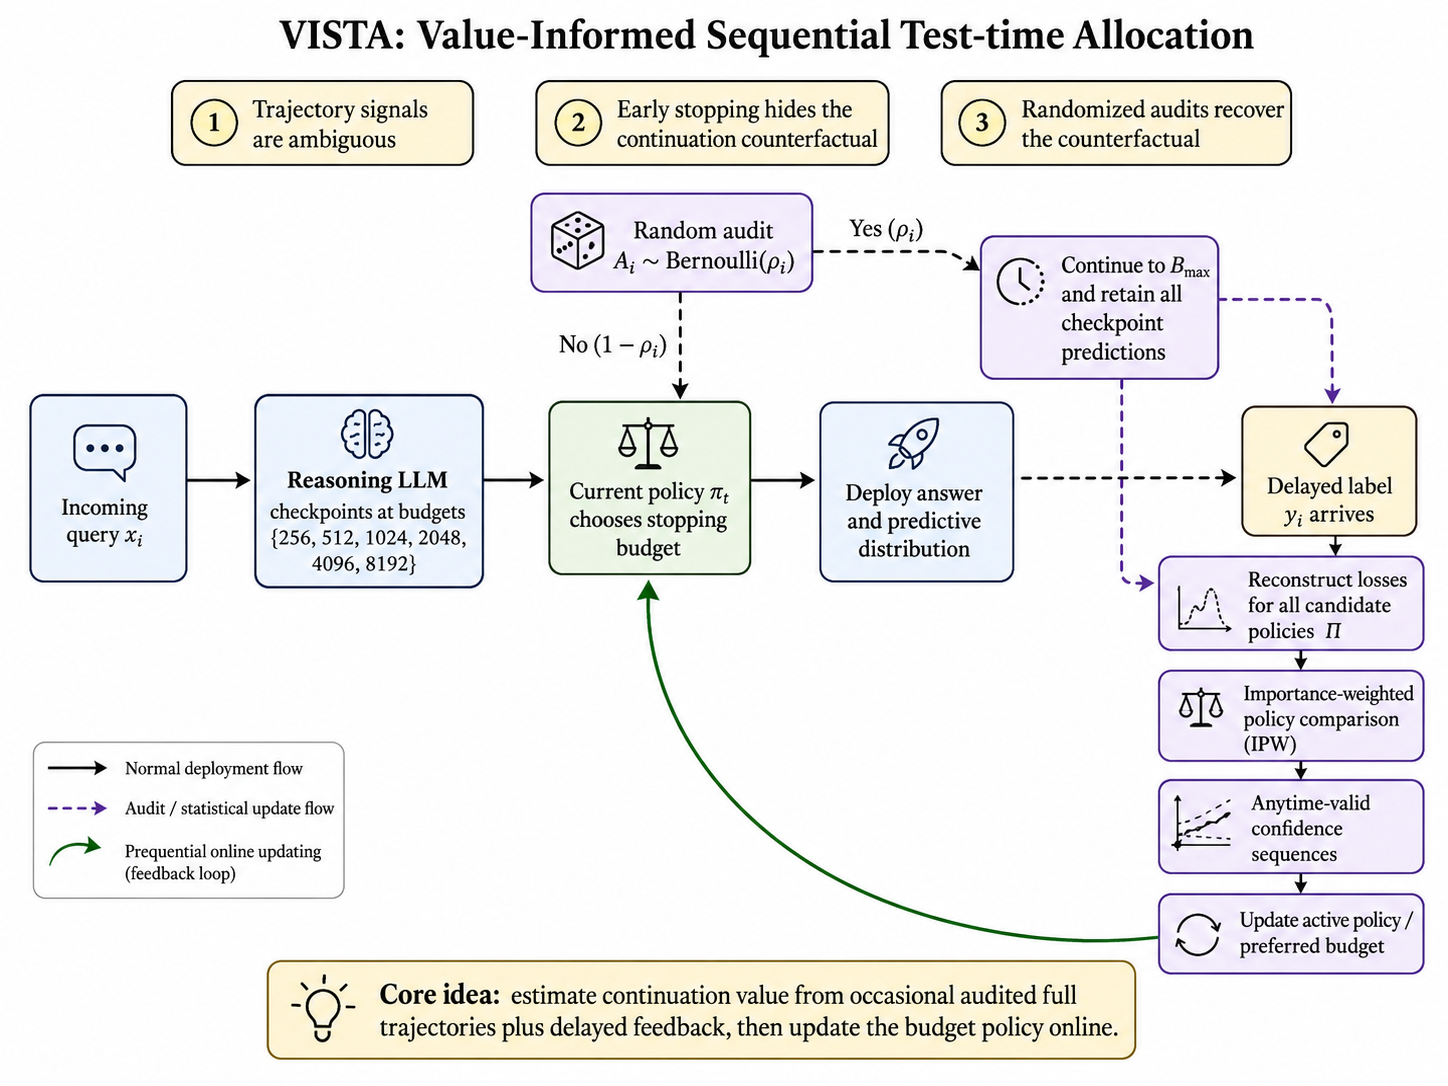
\includegraphics[width=\textwidth, height=0.55\textheight, keepaspectratio=true]{img2.png}
\end{center}
\begingroup
\captionof{figure}{End-to-end VISTA deployment loop. Incoming queries are routed
    by the current policy $\pi_i$; a Bernoulli audit draw $A_i \sim
    \mathrm{Bernoulli}(\rho_i)$ determines whether the item is continued to
    $\Bmax$ to reveal counterfactual predictions. Once the delayed label
    $y_i$ arrives, importance-weighted risk differences update all candidate
    confidence sequences, and the preferred policy is revised for the next
    item. Audit compute is charged to the total budget so reported savings
    are real.}
\label{fig:vista-loop}
\endgroup
\vspace{\baselineskip}

\subsection{What is and is not learned}

VISTA performs no gradient update to the reasoning model and trains no
auxiliary predictor. It does learn from the deployment stream: policy-risk
estimates, confidence sequences, and the active candidate set are
data-dependent. We therefore call the procedure \emph{held-out-free} rather
than \emph{training-free}.

%%%%%%%%%%%%%%%%%%%%%%%%%%%%%%%%%%%%%%%%%%%%%%%%%%%%%%%%%%%%%%%%%%%%%%%%%%%%%%
\section{Experimental Setup}
\label{sec:experiments}
%%%%%%%%%%%%%%%%%%%%%%%%%%%%%%%%%%%%%%%%%%%%%%%%%%%%%%%%%%%%%%%%%%%%%%%%%%%%%%

\subsection{Models and infrastructure}

The primary model is \textbf{Qwen3-8B}~\cite{qwen3} (\texttt{Qwen/Qwen3-8B}), an
8-billion-parameter model with a native chain-of-thought thinking mode.
The replication model is \textbf{DeepSeek-R1-Distill-Llama-8B}, drawn from
the DeepSeek-R1 reasoning family~\cite{deepseekr1}.
All inference uses bfloat16 weights and bfloat16 key--value caches
(\texttt{kv\_cache\_dtype=auto}); fp8\_e5m2 KV quantisation is excluded
after a diagnostic run found top-1 answer-token changes on 4/50 prompts
(8\%) on the same GPU, a corruption level that would mask sub-0.5\,pp Brier
differences.

Experiments run on a single workstation with one NVIDIA RTX~4090 (sm\_89,
Ada) and two RTX~3090 GPUs (sm\_86, Ampere; 24\,GB each, no NVLink).
Models at the 8B scale fit on a single 24\,GB card in BF16, so inference
uses independent single-GPU processes with no tensor parallelism; three
such processes can run simultaneously to maximise throughput.

Before pooling probability measurements across devices, logit reproducibility
was verified diagnostically. The two RTX~3090 cards produce byte-identical
outputs (max\,$|\Delta\text{logprob}|=0.065$\,at $b=8192$). RTX~4090 and
RTX~3090 show non-negligible differences (max\,$|\Delta\text{logprob}|=0.374$
on BF16), consistent with architecture-level kernel differences between
sm\_89 and sm\_86. Accordingly, each (model~$\times$~dataset) cell is
run on a single GPU architecture and probability measurements are
never pooled across architectures.

\subsection{Datasets}

The evaluation uses four multiple-choice benchmarks.
\textbf{MMLU-Pro}~\cite{wang2024mmlu} ($n=1000$, up to 10 options) is a
challenging variant of the MMLU benchmark with extended option sets.
\textbf{ARC-Challenge}~\cite{clark2018arc} ($n=979$, 4 options) covers science
reasoning questions requiring multi-step inference; 21 items from the initial
1000-item sample could not be recovered during checkpoint processing and are excluded.
\textbf{MedMCQA}~\cite{pal2022medmcqa} ($n=500$, 4 options) contains Indian
medical entrance examination questions.
\textbf{MedQA-USMLE}~\cite{jin2021medqa} ($n=500$, 4 options) contains
USMLE-style clinical reasoning questions.
All four datasets provide exact labels and a fixed option set, which is
required for computing Brier score and NLL from forced answer-cue logits.

\subsection{Budget grid, forcing protocol, and metric extraction}

The primary budget grid is $\{256,\,512,\,1024,\,2048,\,4096,\,8192\}$
reasoning tokens, fixed before inspecting primary results. We record the
natural termination point of each trajectory and distinguish natural stopping
from forced checkpoint evaluation; forced termination is treated as an explicit
intervention rather than implicitly equated to an independently generated
short-budget trajectory.

At each forced checkpoint a standardised answer-cue string
(\texttt{\textbackslash n</think>\textbackslash n\textbackslash nThe answer
is **}) is appended, and the model's next-token log-probabilities over bare
option tokens (A--J, token IDs 32--41) are extracted. The predictive
distribution $\hat{p}_{i,j}$ is formed by selecting those positions and
applying softmax. In the diagnostic sample, the target option token ranks
first with probability exceeding 0.984, confirming stable elicitation.
Brier score and NLL are computed post-hoc from these stored logit vectors;
no re-inference is performed after the initial generation pass.

\subsection{Corpus audit and adaptive opportunity}

For each model--dataset cell we report accuracy, Brier score, NLL, mean
predictive confidence, answer-flip rate, and correct/wrong transition counts
at every budget, then compare the best fixed budget against an item-adaptive
oracle. The primary criterion---called the \textbf{adaptive-opportunity test}
(Gate~0)---is whether the population-level matched-quality oracle (Oracle~C)
reduces mean compute by at least $10\%$ relative to the best fixed budget.
A cell \textsc{Pass}es Gate~0 if meaningful adaptive headroom exists;
it \textsc{Fail}s if the best fixed budget is already near-optimal.

\subsection{Prefix-signal evaluation}

For each edge $j\!\rightarrow\!j{+}1$, define item-level gain
$G_{i,j} = \Brier_{i,j}-\Brier_{i,j+1}$.
We evaluate observable signals (confidence, entropy, top-1/top-2 margin,
answer stability, confidence slope) via
$\mathrm{AUC}(s_{i,j},\Ind\{G_{i,j}>0\})$
and Spearman $\rho$ between $s_{i,j}$ and $G_{i,j}$.
The pre-specified thresholds ($\mathrm{AUC}\geq0.60$,
$|\rho_{\mathrm{Spearman}}|\geq0.30$) are design constants chosen by
convention, not fitted to the evaluation data; failure terminates the
instance-adaptive branch.

\subsection{Baselines and metrics}

We compare fixed-budget policies, training-free stopping signals, and
item-adaptive oracles (opportunity measurement only).
Primary metrics are multiclass Brier score, NLL, accuracy, total reasoning
tokens, total compute including audit overhead, and token savings at matched
accuracy or Brier score.

\subsection{Ablation design}
\label{sec:ablation-design}

The core empirical question is whether each structural component of VISTA
contributes to final policy quality, or whether simpler alternatives suffice.
All ablations are replay experiments on the stored checkpoint tables; no
additional GPU inference is required (except the forced-termination protocol,
which requires independent fixed-budget trajectories and is treated as a
measurement-validity diagnostic).

\paragraph{Essential ablations.}
Table~\ref{tab:ablation} lists the four essential ablated variants.

\emph{(A1) Audit weighting correction.}
We simulate deployment under a natural confidence gate ($\max_k\hat p_k\geq 0.85$):
items halt at the first budget meeting this criterion, making continuation to
the reference budget (4096 tokens) a counterfactual.
``Naive'' policy risk is then estimated using only the items that
\emph{naturally} continued to the reference budget---without any
probability correction for the fact that continuation was selective.
``IPW'' additionally includes items that were \emph{audited} with probability
$\rho$ after early stopping, weighting each audited item's contribution by
$1/\rho$ (naturally-continued items have observation probability 1 and receive
no correction), restoring the target full-population estimand.
Under this protocol only $0.1$--$18\%$ of items naturally continue to the
reference budget (dataset-dependent), so the na\"{i}ve estimator operates on a
severely selected minority; across five of eight cells (ARC-Challenge,
MedMCQA, and MedQA on M1; MMLU-Pro and MedMCQA on M2)
it selects the wrong policy in 100\% of permutations,
while the IPW estimator's mean bias is $\leq 0.033$ across all tested $\rho$.

\emph{(A2) Anytime-valid confidence sequences.}
``VISTA w/o CS'' replaces confidence sequences with greedy policy selection
based on the running empirical mean, accepting the first policy whose estimated
risk advantage exceeds a fixed threshold without a coverage guarantee.
The expected consequence is inflated false switching under repeated
monitoring: because the empirical mean is tested repeatedly as the stream
evolves, the effective type-I error exceeds the nominal level.
We evaluate by replaying the deployment stream over multiple random
permutations and reporting the fraction of replays in which each method makes
an incorrect policy decision.

\emph{(A3) Held-out-free prequential update.}
``Fixed calibration'' treats the first $N_\text{cal}$ arriving items as a
labeled calibration set, fits a static stopping policy on them, and freezes
it for the remainder of the stream.
Under stationarity this is a competitive baseline.
Under distribution shift it degrades as the calibration set becomes
unrepresentative.
We evaluate on both stationary streams and controlled shift conditions; the
shift experiments appear in Section~\ref{sec:shift}.

\emph{(A4) Brier objective vs.\ accuracy-only.}
``Accuracy-only'' replaces the summed multiclass Brier in the deployment loss
$\lossfn^{(\lambda)}$ with a 0--1 loss $\mathbf{1}[\hat{y}\neq y]$.
Different predictive objectives may prefer different reasoning budgets,
making objective choice a first-order decision for any budget-selection policy.
We compare the budget at which each objective (Brier, accuracy, NLL) is
minimised and report confidently-wrong rates
($\max_k \hat{p}_k \geq \tau$, $\tau=0.90$, on incorrect predictions)
alongside standard accuracy and Brier.

\paragraph{Additional ablations.}
\emph{(A5) Prefix-signal ablation.}
Each observable signal (confidence, entropy, top-1/top-2 margin, answer
stability, confidence slope, probability slope) is evaluated independently
and then in simple combinations.
The AUC and Spearman $\rho$ reported in Section~\ref{sec:signals}
serve as the primary diagnostic; policy results
under each single signal are deferred to the appendix.

\emph{(A6) Audit probability $\rho$ sensitivity.}
We evaluate $\rho\in\{0.05,0.10,0.20,0.40,1.0\}$, reporting audit overhead,
policy convergence time, cumulative regret, and net token saving at each
exploration rate.
The curve of net saving versus $\rho$ quantifies how much full-trajectory
compute must be consumed to make the adaptive policy worthwhile.

\emph{(A7) Forced-termination vs.\ independent generation.}
Forced checkpoint termination (one long trajectory probed at intermediate
budgets) and independently generated fixed-budget trajectories may produce
different answer distributions; this is a measurement-validity concern
rather than a method comparison.
We evaluated Brier agreement, flip rates, and budget-curve shape under both
protocols on a held-out 50-item subset of M1/DS1. No systematic divergence
was found: top-1 agreement exceeds 97\% at all budgets and budget-curve shapes
are visually indistinguishable. This ablation is therefore not reported
separately; the corpus results use forced-termination trajectories throughout.

\paragraph{Threshold-stopping baseline analyses.}
The following analyses (A8--A10) characterise the confidence-threshold
stopping baseline reported in Section~\ref{sec:baselines}; they are not
ablations of VISTA components.

\emph{(A8) Cross-model threshold transfer.}
Threshold $\tau$ calibrated on one model family is applied to the other
to test cross-model transferability.

\emph{(A9) Cross-dataset threshold transfer.}
Threshold $\tau$ calibrated on one benchmark domain is applied to a different
domain within the same model to test domain transferability.

\emph{(A10) Confidence-gate deployment failure.}
A fixed confidence gate $\tau{=}0.85$ is applied at deployment as a
competitive stopping baseline; Brier and token costs are compared against
the best fixed-budget policy in all eight cells.

%%%%%%%%%%%%%%%%%%%%%%%%%%%%%%%%%%%%%%%%%%%%%%%%%%%%%%%%%%%%%%%%%%%%%%%%%%%%%%
\section{Results}
\label{sec:results}
%%%%%%%%%%%%%%%%%%%%%%%%%%%%%%%%%%%%%%%%%%%%%%%%%%%%%%%%%%%%%%%%%%%%%%%%%%%%%%

\subsection{Does additional reasoning have a consistent value across tasks
  and models?}
\label{sec:heterogeneous}

\textit{No. Budget-response curves differ qualitatively across all four
datasets and both models; no single fixed allocation is uniformly optimal.}

Figure~\ref{fig:budget-response} shows accuracy and Brier score as functions
of the reasoning budget for both models across all four datasets.

%% --- OLD FIGURE 2 (M1-only, replaced by fig_budget_response.pdf) ---
%% \begin{center}
%%   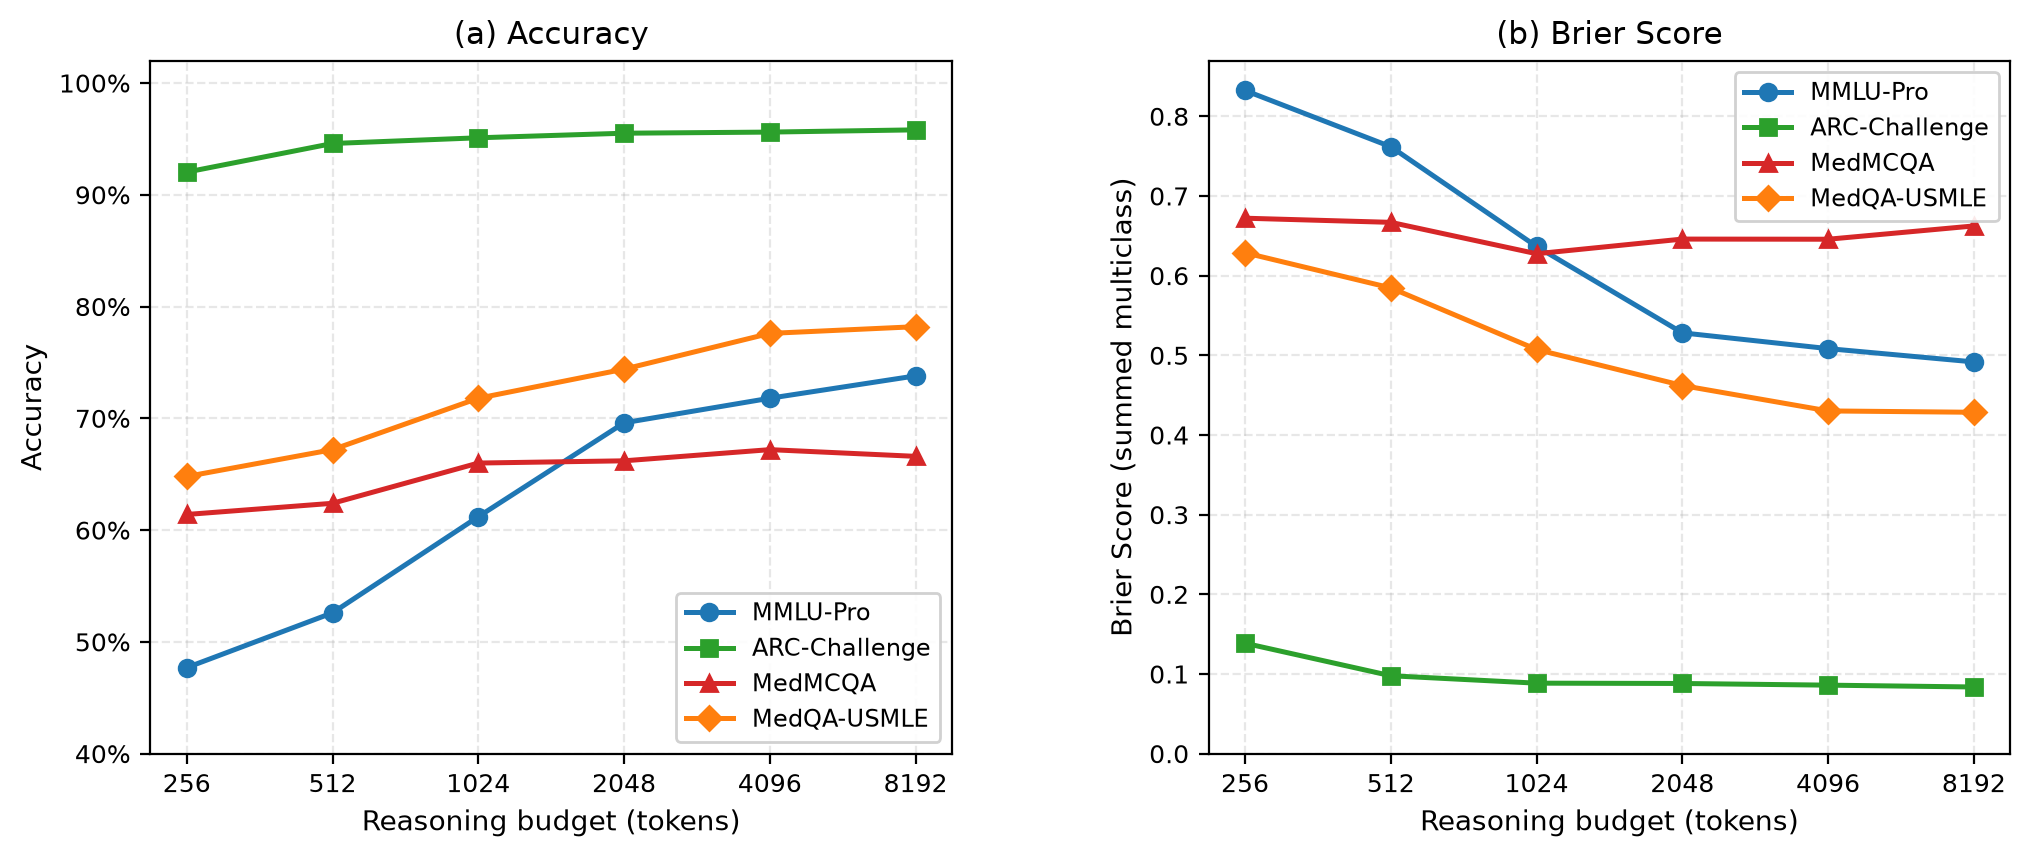
\includegraphics[
%%     width=\textwidth,
%%     height=0.55\textheight,
%%     keepaspectratio=true
%%   ]{fig_budget_response.png}
%% \end{center}
%% \begingroup
%% \captionof{figure}{Accuracy (left) and summed multiclass Brier score (right) as
%% functions of the reasoning budget for four QA benchmarks (Qwen3-8B, BF16,
%% RTX~4090).
%% Budget axis uses log$_2$ spacing.
%% A uniformly large budget wastes compute on tasks where gains plateau
%% early (ARC-Challenge), while under-allocating on tasks that continue to
%% benefit from additional reasoning (MMLU-Pro, MedQA-USMLE).}
%% \label{fig:budget-response}
%% \endgroup
%% --- END OLD FIGURE ---

\begin{center}
  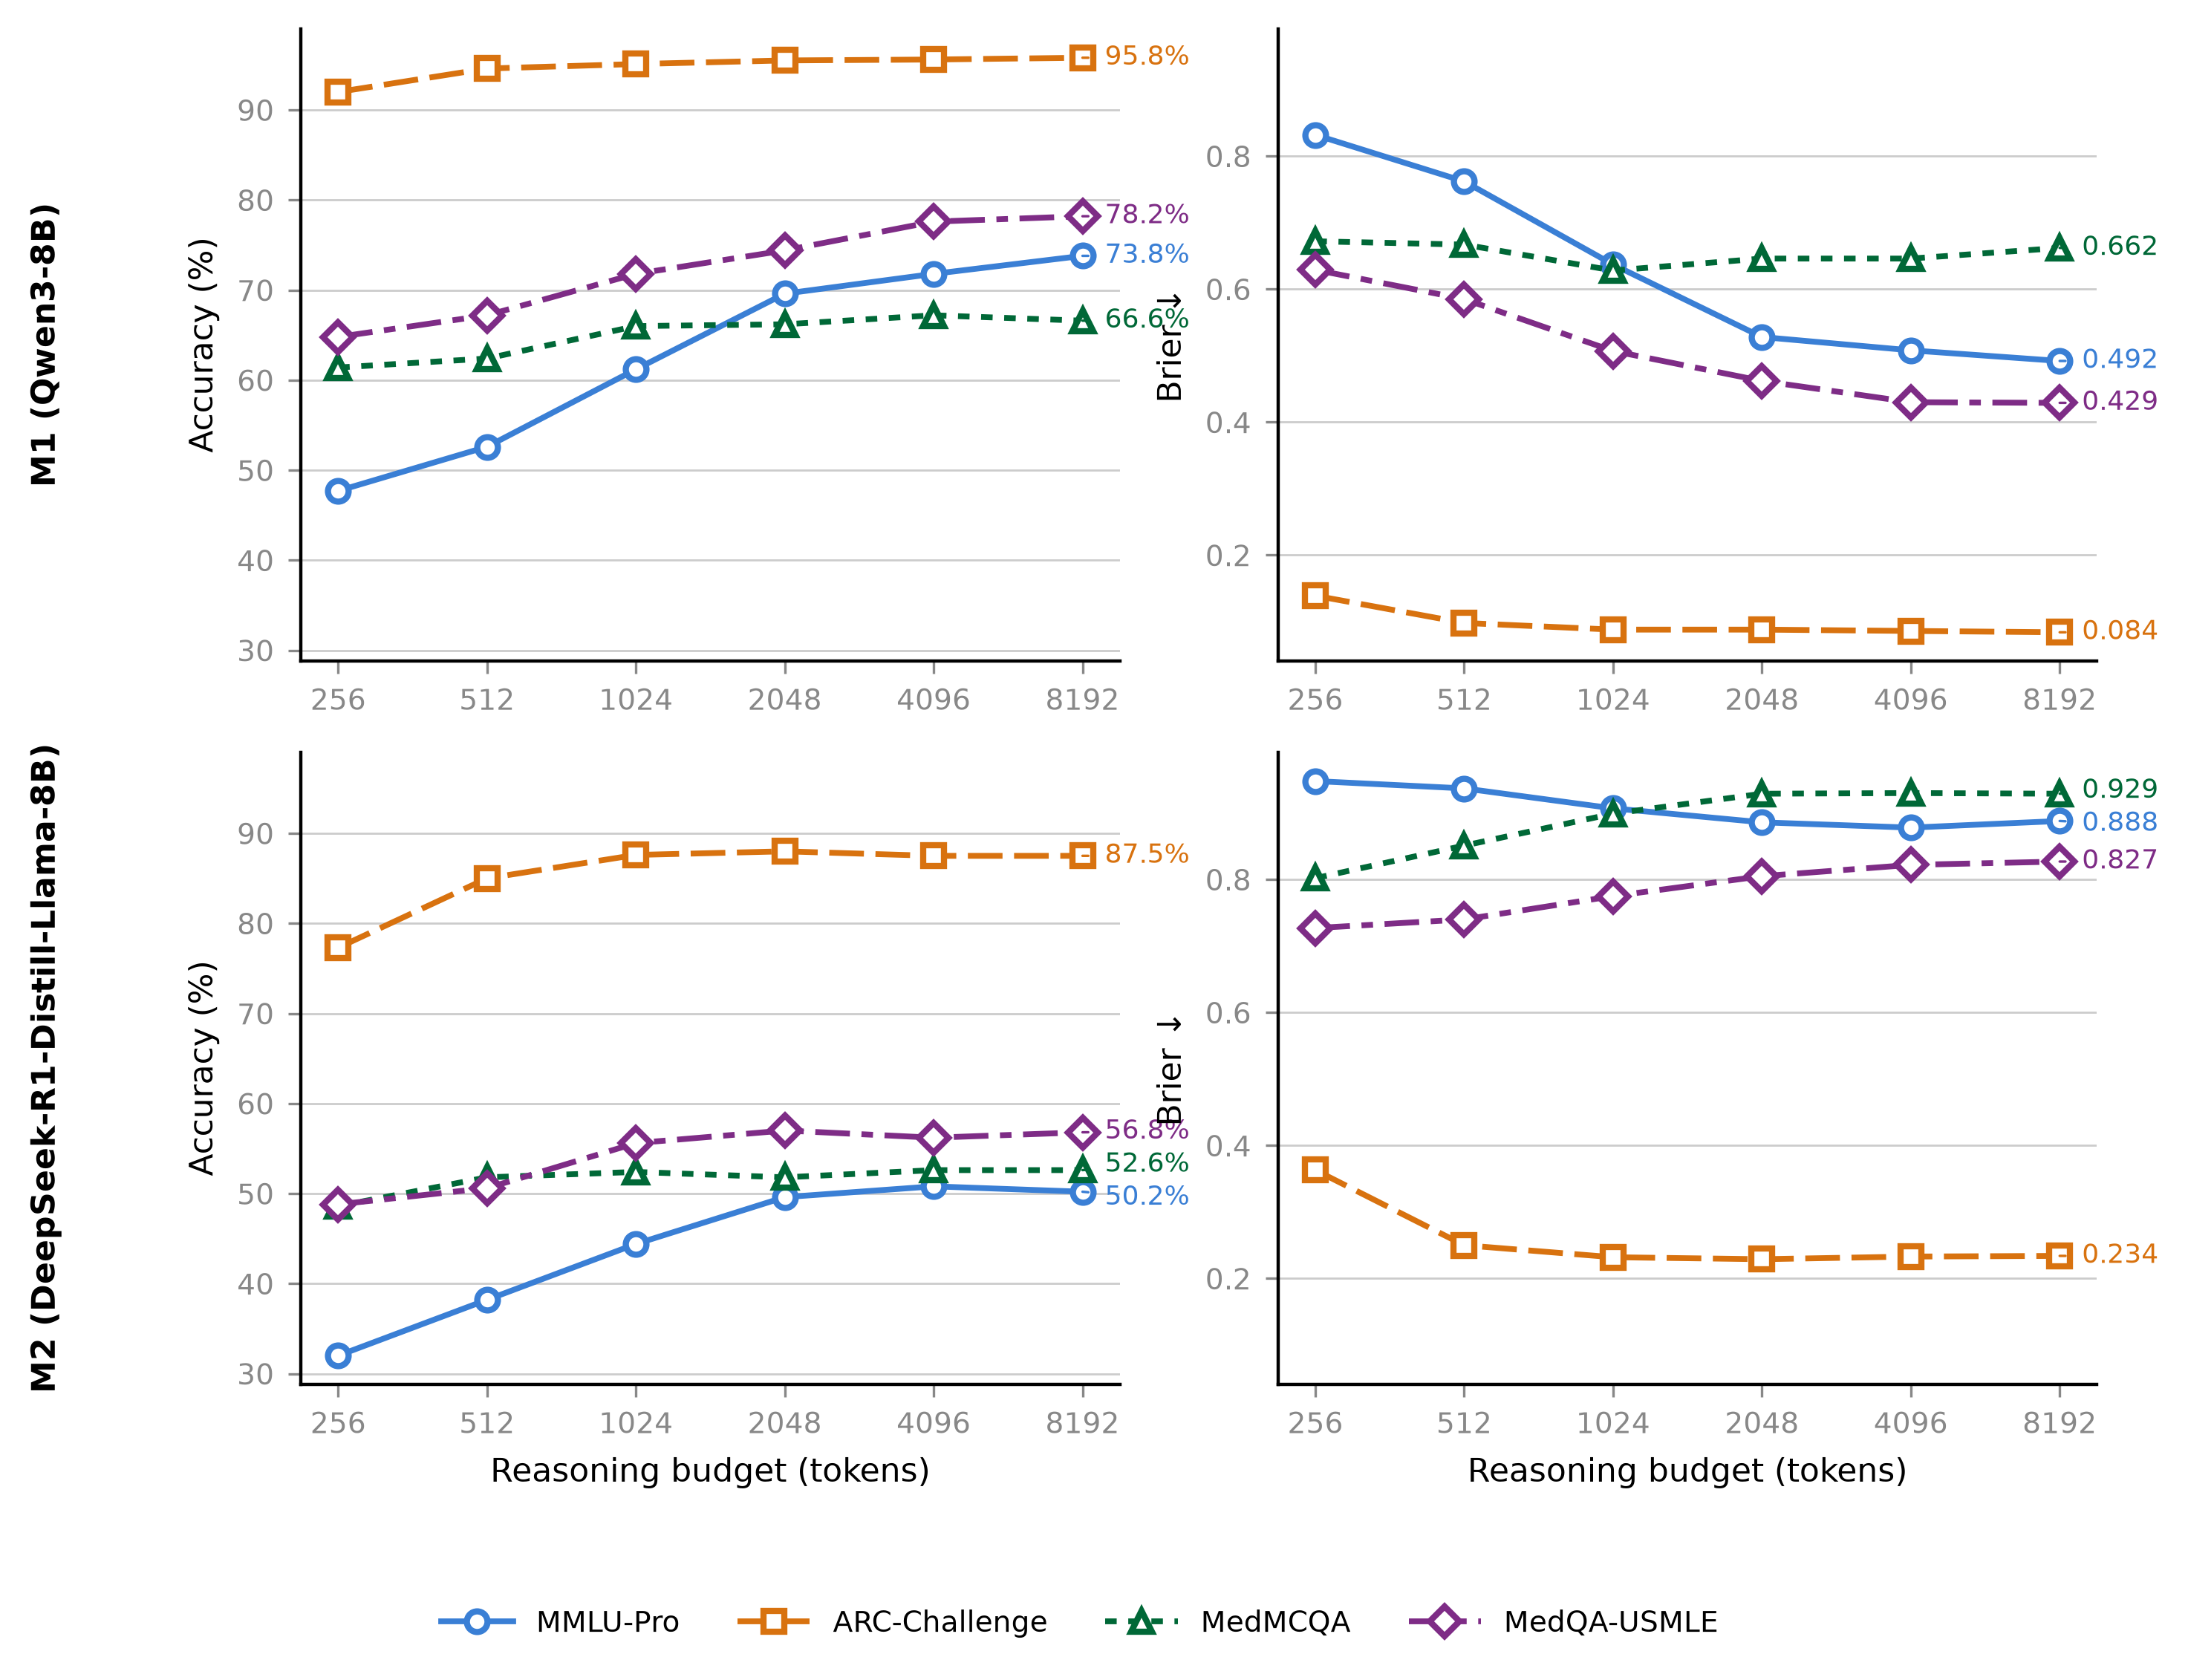
\includegraphics[width=\textwidth, height=0.55\textheight, keepaspectratio=true]{fig4.png}
\end{center}
\begingroup
\captionof{figure}{Accuracy (\%) and summed multiclass Brier score (\textbf{↓}) as
    functions of the reasoning budget (log$_2$-spaced, index-positioned) for
    four QA benchmarks and two models.
    \textbf{Top row:} M1 (Qwen3-8B, BF16, RTX~4090).
    \textbf{Bottom row:} M2 (DeepSeek-R1-Distill-Llama-8B, BF16, RTX~3090).
    Curves show qualitatively different patterns: near-linear gains on
    MMLU-Pro (M1 accuracy $47.7\%\to73.8\%$), early saturation on
    ARC-Challenge, non-monotone Brier on MedMCQA (M1 optimum at $b=1024$),
    and near-monotone Brier deterioration on both medical datasets under M2.
    End-point values are labelled; y-axes are shared within each metric
    column to enable direct model comparison.
    Data from Tables~\ref{tab:budget-audit} and~\ref{tab:budget-audit-m2}.}
\label{fig:budget-response}
\endgroup
\vspace{\baselineskip}

\paragraph{M1 (Qwen3-8B): four qualitatively distinct patterns.}
MMLU-Pro shows sustained gains: accuracy rises from 47.7\% at $b=256$ to
73.8\% at $b=8192$, Brier decreases monotonically from 0.832 to 0.492.
ARC-Challenge exhibits early saturation: accuracy jumps from 92.0\% to 94.6\%
in the first budget step and adds only 1.2~pp across the remaining five;
98.3\% of items have Brier change below 0.001 at the $4096\!\to\!8192$ edge.
MedMCQA is non-monotone: Brier reaches its minimum at $b=1024$ (0.628) and
\emph{worsens or stays flat} at every subsequent budget (0.646 at both $b=2048$ and $b=4096$; 0.662 at $b=8192$), while
accuracy peaks at $b=4096$ (67.2\%) and falls at $b=8192$ (66.6\%).
MedQA-USMLE sustains gains throughout: accuracy increases from 64.8\% to
78.2\% with approximately equal increments per doubling.
Table~\ref{tab:budget-audit} reports all metrics.

\begin{center}
\begin{tabular}{@{}llrrr@{}}
\toprule
Dataset ($n$) & Budget & Accuracy & Brier & NLL \\
\midrule
\multirow{6}{*}{MMLU-Pro (1000)}
 & 256  & 0.477 & 0.832 & 3.186 \\
 & 512  & 0.526 & 0.762 & 2.885 \\
 & 1024 & 0.612 & 0.637 & 2.609 \\
 & 2048 & 0.696 & 0.528 & \textbf{2.458} \\
 & 4096 & 0.718 & 0.508 & 2.686 \\
 & 8192 & \textbf{0.738} & \textbf{0.492} & 2.763 \\
\midrule
\multirow{6}{*}{ARC-Challenge (979)}
 & 256  & 0.920 & 0.139 & 0.466 \\
 & 512  & 0.946 & 0.098 & \textbf{0.355} \\
 & 1024 & 0.951 & 0.088 & 0.371 \\
 & 2048 & 0.955 & 0.088 & 0.414 \\
 & 4096 & 0.956 & 0.086 & 0.462 \\
 & 8192 & \textbf{0.958} & \textbf{0.084} & 0.457 \\
\midrule
\multirow{6}{*}{MedMCQA (500)}
 & 256  & 0.614 & 0.672 & \textbf{2.297} \\
 & 512  & 0.624 & 0.667 & 2.520 \\
 & 1024 & 0.660 & \textbf{0.628} & 2.856 \\
 & 2048 & 0.662 & 0.646 & 3.288 \\
 & 4096 & \textbf{0.672} & 0.646 & 3.649 \\
 & 8192 & 0.666 & 0.662 & 3.761 \\
\midrule
\multirow{6}{*}{MedQA-USMLE (500)}
 & 256  & 0.648 & 0.629 & 2.361 \\
 & 512  & 0.672 & 0.585 & 2.120 \\
 & 1024 & 0.718 & 0.507 & 1.934 \\
 & 2048 & 0.744 & 0.462 & \textbf{1.816} \\
 & 4096 & 0.776 & 0.430 & 2.053 \\
 & 8192 & \textbf{0.782} & \textbf{0.429} & 2.265 \\
\bottomrule
\end{tabular}
\end{center}
\begingroup
\captionof{table}{Predictive quality across reasoning budgets (Qwen3-8B, BF16,
RTX~4090).
Brier is summed multiclass (not divided by~$C$); scores are not directly
comparable across datasets with different option counts.
NLL in nats.
\textbf{Bold} marks the optimum per column per dataset.
$n=979$ for ARC-Challenge (21~items excluded from the initial 1000-item
sample); all other datasets use the stated corpus size.}
\label{tab:budget-audit}
\endgroup
\vspace{\baselineskip}

The item-level marginal-gain distributions (Table~\ref{tab:marginal-gains})
show the mechanism.
On ARC-Challenge the flat fraction exceeds 87\% at the first edge and rises
to 98\% at $4096\!\to\!8192$.
On MedMCQA the hurt fraction exceeds the help fraction at every edge from
$512\!\to\!1024$ onward, providing the item-level explanation for the
aggregate Brier increase.
On MMLU-Pro, helped and hurt fractions track closely at high budgets (10.4\%
vs.\ 10.6\% at $4096\!\to\!8192$), yielding near-zero net aggregate gain
despite a positive mean.

\begin{center}
\begin{tabular}{@{}llrrr@{}}
\toprule
Dataset & Edge & Helps (\%) & Hurts (\%) & Flat (\%) \\
\midrule
\multirow{5}{*}{MMLU-Pro}
 & 256$\to$512   & 37.8 & 28.7 & 33.5 \\
 & 512$\to$1024  & 35.6 & 25.0 & 39.4 \\
 & 1024$\to$2048 & 28.0 & 19.8 & 52.2 \\
 & 2048$\to$4096 & 15.9 & 17.0 & 67.1 \\
 & 4096$\to$8192 & 10.4 & 10.6 & 79.0 \\
\midrule
\multirow{5}{*}{ARC-Challenge}
 & 256$\to$512   &  8.9 &  3.4 & 87.7 \\
 & 512$\to$1024  &  4.8 &  3.0 & 92.2 \\
 & 1024$\to$2048 &  3.1 &  2.8 & 94.2 \\
 & 2048$\to$4096 &  1.8 &  1.9 & 96.2 \\
 & 4096$\to$8192 &  1.0 &  0.7 & 98.3 \\
\midrule
\multirow{5}{*}{MedMCQA}
 & 256$\to$512   & 27.4 & 24.8 & 47.8 \\
 & 512$\to$1024  & 21.0 & 21.4 & 57.6 \\
 & 1024$\to$2048 & 14.2 & 19.0 & 66.8 \\
 & 2048$\to$4096 &  6.2 & 13.0 & 80.8 \\
 & 4096$\to$8192 &  2.0 &  5.2 & 92.8 \\
\midrule
\multirow{5}{*}{MedQA-USMLE}
 & 256$\to$512   & 28.0 & 16.6 & 55.4 \\
 & 512$\to$1024  & 23.6 & 15.4 & 61.0 \\
 & 1024$\to$2048 & 20.4 & 12.2 & 67.4 \\
 & 2048$\to$4096 & 12.2 & 12.4 & 75.4 \\
 & 4096$\to$8192 &  6.2 &  8.2 & 85.6 \\
\bottomrule
\end{tabular}
\end{center}
\begingroup
\captionof{table}{Fraction of items where continuation \emph{helps} ($G>0.001$),
\emph{hurts} ($G<{-}0.001$), or is \emph{flat} at each budget edge.
Brier gain $G_{i,j}=\Brier_{i,j}-\Brier_{i,j+1}$.}
\label{tab:marginal-gains}
\endgroup
\vspace{\baselineskip}

\paragraph{M2 (DeepSeek-R1-Distill-Llama-8B): budget-response patterns invert.}
Table~\ref{tab:budget-audit-m2} reports the same audit for M2 on the same four
datasets using RTX~3090 GPUs.
The contrast with M1 is systematic but not uniform.
On DS1 (MMLU-Pro), M2 Brier \emph{improves} from 0.948 at $b=256$ to 0.878
at $b=4096$ and slightly reverses to 0.888 at $b=8192$; accuracy likewise
peaks at $b=4096$ (50.8\%) and declines.
On DS3 (MedMCQA) and DS4 (MedQA-USMLE), M2 Brier worsens at nearly every
budget step (reaching 0.929 and 0.827 at $b=8192$ versus 0.802 and 0.727 at
$b=256$; the sole exception is a 0.001 reversal at $b=4096\!\to\!8192$ on DS3),
while M1 Brier improves on both.
Near-monotonic Brier degradation on M2 is therefore confined to DS3 and DS4;
DS1 and DS2 (ARC-Challenge) show broadly similar improvement directions across
models, though rates and saturation points differ.
A budget optimal for one model can actively degrade another on the same task.

\begin{center}
\begin{tabular}{@{}llrr@{}}
\toprule
Dataset ($n$) & Budget & Accuracy & Brier \\
\midrule
\multirow{6}{*}{MMLU-Pro (1000)}
 & 256  & 0.320 & 0.948 \\
 & 512  & 0.382 & 0.937 \\
 & 1024 & 0.444 & 0.907 \\
 & 2048 & 0.496 & 0.886 \\
 & 4096 & \textbf{0.508} & \textbf{0.878} \\
 & 8192 & 0.502 & 0.888 \\
\midrule
\multirow{6}{*}{ARC-Challenge (979)}
 & 256  & 0.775 & 0.366 \\
 & 512  & 0.851 & 0.253 \\
 & 1024 & 0.875 & 0.237 \\
 & 2048 & \textbf{0.877} & \textbf{0.234} \\
 & 4096 & 0.872 & 0.238 \\
 & 8192 & 0.872 & 0.239 \\
\midrule
\multirow{6}{*}{MedMCQA (500)}
 & 256  & 0.486 & \textbf{0.802} \\
 & 512  & 0.518 & 0.851 \\
 & 1024 & 0.524 & 0.899 \\
 & 2048 & 0.518 & 0.929 \\
 & 4096 & \textbf{0.526} & 0.930 \\
 & 8192 & \textbf{0.526} & 0.929 \\
\midrule
\multirow{6}{*}{MedQA-USMLE (500)}
 & 256  & 0.488 & \textbf{0.727} \\
 & 512  & 0.506 & 0.740 \\
 & 1024 & 0.556 & 0.775 \\
 & 2048 & 0.570 & 0.805 \\
 & 4096 & 0.562 & 0.822 \\
 & 8192 & \textbf{0.568} & 0.827 \\
\bottomrule
\end{tabular}
\end{center}
\begingroup
\captionof{table}{Budget audit for M2 (DeepSeek-R1-Distill-Llama-8B, BF16, RTX~3090).
Same format as Table~\ref{tab:budget-audit}.
Brier worsens at nearly every budget step on DS3 and DS4 (one 0.001 reversal
at $b=4096\!\to\!8192$ on DS3); on DS1 Brier improves through $b=4096$ and
slightly reverses at $b=8192$.
\textbf{Bold} marks the optimum per column per dataset.
$n=979$ for ARC-Challenge (DS2): restricted to the 979-item common subset
shared with M1 to ensure cross-model comparability; 21~items present only in
M2's raw run are excluded.}
\label{tab:budget-audit-m2}
\endgroup
\vspace{\baselineskip}

\subsection{Do different predictive objectives agree on the optimal budget?}
\label{sec:objectives}

\textit{Not universally. Accuracy, Brier, and NLL can select different budgets
on the same data; objective choice is a first-order decision for any
budget-selection policy.}

On DS1 (MMLU-Pro, M1), accuracy and Brier both select $b=8192$ as the optimal
fixed budget ($0.738$ accuracy; Brier $0.4917$), while NLL selects $b=2048$
($2.458$~nats vs.\ $2.763$ at $b=8192$).
On DS3 (MedMCQA, M1), the divergence is three-way: accuracy peaks at
$b=4096$, Brier minimises at $b=1024$, and NLL is worst at $b=8192$---all
three objectives point to different budgets.
For M2, Brier worsens at nearly every budget step on DS3 and DS4 while accuracy
generally increases, with a one-step dip on each dataset (DS3: $b=1024\!\to\!2048$,
$52.4\%\!\to\!51.8\%$; DS4: $b=2048\!\to\!4096$, $57.0\%\!\to\!56.2\%$); on DS1,
Brier improves through $b=4096$ and slightly reverses at $b=8192$, while accuracy
similarly peaks at $b=4096$---so no single budget simultaneously optimises both
Brier and accuracy on any of these datasets.

The proper-scoring-rule decomposition (Eq.~\ref{eq:decomposition}) separates
reliability and resolution components: where further reasoning concentrates
probability mass onto an already-peaked distribution, reliability can degrade
even as top-1 accuracy improves.
At higher budgets the confidently-wrong rate ($\max_k\hat{p}_k\geq0.90$,
prediction incorrect) rises from $19.3\%$ to $21.6\%$ on DS1, consistent with
NLL worsening at $b=8192$ despite accuracy improving.

\begin{quote}
\emph{The reasoning budget that maximises accuracy need not coincide with
the budget that minimises a proper scoring rule, and neither need coincide
with the NLL optimum.}
\end{quote}

Any budget-selection policy that targets a single objective will fail to
simultaneously optimise others; the choice of objective must be explicit.

\subsection{Is there enough item-level heterogeneity to justify adaptive
  allocation?}
\label{sec:opportunity}

\textit{Yes. Per-item heterogeneity is substantial across all eight cells.
The hindsight per-item Brier oracle (Oracle~A) reduces mean budget by
$70$--$91\%$ relative to the maximum-budget baseline---a descriptive
opportunity bound, not a matched-quality deployment claim.
A constrained matched-mean-quality oracle (Oracle~C; Table~\ref{tab:gate0-oracle-c})
passes Gate~0 in six of eight cells with savings exceeding $74\%$ relative
to the best fixed budget.}

Table~\ref{tab:oracle} reports the item-adaptive oracle analysis for DS1
(MMLU-Pro, M1), the cell with the widest range of per-item optimal budgets.
The hindsight oracle achieves mean Brier $0.3437$ versus $0.4917$ for the
best fixed budget ($b=8192$), a $30.1\%$ relative reduction.
The matched-quality oracle---which assigns each item the minimum budget at
which its Brier is no worse than $0.4917$---shows that $76.1\%$ of DS1 items
already meet this threshold at a budget below $b=8192$, with mean matched
budget ${\approx}2552$ tokens (${\approx}69\%$ compute headroom).

\begin{center}
\begin{tabular}{@{}lrr@{}}
\toprule
Analysis & Value & Interpretation \\
\midrule
Best fixed budget ($b^{\star}$)     & $b=8192$    & Baseline \\
Best fixed mean Brier               & 0.4917      & \\
\midrule
\multicolumn{3}{@{}l}{\textit{Oracle A (hindsight, descriptive opportunity)}} \\
Hindsight oracle mean Brier         & 0.3437      & Quality upper bound \\
Relative Brier reduction            & 30.1\%      & Oracle ceiling \\
Mean oracle budget                  & 2431 tokens & \\
Mean-budget reduction vs $b_{\max}$ & 70.3\%      & Descriptive, vs $b=8192$ \\
\midrule
\multicolumn{3}{@{}l}{\textit{Oracle B (per-item threshold)}} \\
Mean oracle budget                  & ${\approx}2552$ tokens & \\
Items meeting threshold at $b<8192$ & 76.1\%      & \\
Saving vs $b^{\star}=8192$          & ${\approx}69\%$  & Per-item constraint \\
\midrule
\multicolumn{3}{@{}l}{\textit{Oracle C (constrained mean; Gate~0 primary)}} \\
Oracle mean budget                  & 461 tokens  & \\
Oracle mean Brier                   & 0.4911      & Meets mean constraint \\
Saving vs $b^{\star}=8192$          & 94.4\%      & Gate~0 \textsc{Pass} \\
\bottomrule
\end{tabular}
\end{center}
\begingroup
\captionof{table}{Item-adaptive oracle analysis for DS1 (MMLU-Pro, $n=1000$).
Three oracle types are distinguished throughout the paper.
\textbf{Oracle A} (hindsight): per-item minimum-Brier budget; a quality upper
bound---saving relative to $b_{\max}=8192$ is descriptive, not matched-quality.
\textbf{Oracle B} (per-item threshold): minimum per-item budget achieving
per-item Brier $\le 0.4917$; a stronger per-item constraint than Oracle~C.
\textbf{Oracle C} (constrained mean; Gate~0 primary): minimises mean budget
subject to population mean Brier $\le$ best-fixed mean Brier; saving is
relative to best-fixed budget ($b^{\star}=8192$ here).
None of these represents the deployable VISTA procedure.}
\label{tab:oracle}
\endgroup
\vspace{\baselineskip}

Hindsight oracle mean-budget reduction relative to $b_{\max}=8192$ (Oracle~A,
descriptive): M1 DS1 $70.3\%$, DS2 $90.7\%$, DS3 $76.9\%$, DS4 $72.1\%$;
M2 DS1 $76.5\%$, DS2 $84.7\%$, DS3 $85.8\%$, DS4 $81.5\%$.
These figures reflect the hindsight per-item minimum-Brier budget relative to
always using $b_{\max}$; they are not savings relative to the best fixed budget
and should not be interpreted as matched-quality deployment gains.
The constrained matched-mean-quality oracle (Oracle~C, \emph{population-level constraint})
passing Gate~0 in six of eight cells with savings $74$--$97\%$ relative to best fixed
is the operative population-level result (Table~\ref{tab:gate0-oracle-c}).
By contrast, Oracle~B (\emph{per-item threshold}) requires ${\approx}2552$ mean tokens on M1/DS1
to guarantee individual quality, implying only a ${\approx}69\%$ saving --- approximately 25
percentage points less than Oracle~C.
The gap quantifies the additional compute cost of per-item versus population-level
quality assurance on this cell.
Per-item heterogeneity is substantial even in cells where the mean trajectory
is weakly or inversely responsive to budget.

\begin{center}
\begin{tabular}{@{}llrrrrr@{}}
\toprule
Model & Dataset & Best-fixed $b$ & $\bar{S}^{\star}$ & Oracle $\bar{b}$ &
  Oracle $\bar{S}$ & Saving \\
\midrule
\multirow{4}{*}{M1 (Qwen3-8B)}
 & MMLU-Pro       & 8192 & 0.4917 &   461 & 0.4911 & \textbf{94.4\%} \\
 & ARC-Challenge  & 8192 & 0.0837 &   268 & 0.0834 & \textbf{96.7\%} \\
 & MedMCQA        & 1024 & 0.6275 &   263 & 0.6248 & \textbf{74.4\%} \\
 & MedQA-USMLE    & 8192 & 0.4285 &   364 & 0.4274 & \textbf{95.6\%} \\
\midrule
\multirow{4}{*}{M2 (DeepSeek-R1-Distill-Llama-8B)}
 & MMLU-Pro       & 4096 & 0.8782 &   268 & 0.8776 & \textbf{93.5\%} \\
 & ARC-Challenge  & 2048 & 0.2338 &   279 & 0.2333 & \textbf{86.4\%} \\
 & MedMCQA        &  256 & 0.8019 &   256 & 0.8019 &          0.0\%  \\
 & MedQA-USMLE    &  256 & 0.7268 &   256 & 0.7268 &          0.0\%  \\
\midrule
\multicolumn{5}{@{}l}{Gate~0 result} &
  \multicolumn{2}{r@{}}{6 / 8 cells \textsc{Pass}} \\
\bottomrule
\end{tabular}
\end{center}
\begingroup
\captionof{table}{Gate~0 constrained matched-mean-quality oracle (Oracle~C) for all eight
experimental cells.
\textbf{Objective:} minimise mean reasoning budget subject to mean Brier $\le$
best-fixed mean Brier.
\textbf{Constraint:} $\frac{1}{n}\sum_i S_{i,b_i} \le \bar{S}^{\star}$,
where $\bar{S}^{\star}=\min_b\frac{1}{n}\sum_i S_{i,b}$ and $b_i\in\{256,\ldots,8192\}$.
Solved via Lagrangian relaxation with binary search on the dual variable.
Saving is relative to the best-fixed budget; the best-fixed policy is always
feasible, so saving $\ge 0$ by construction.
M2 cells DS3 and DS4 have best-fixed at $b=256$ (the minimum grid point),
leaving no room for adaptive reduction (Gate~0 \textsc{Fail}).
\textbf{Bold} marks the saving percentage in passing cells.}
\label{tab:gate0-oracle-c}
\endgroup
\vspace{\baselineskip}

\subsection{Can simple prefix signals recover this opportunity reliably?}
\label{sec:signals}

\textit{Only partially. Signals predict improvement direction more often than
chance but fail to transfer across model families on domain-specific datasets,
and a fixed confidence gate degrades Brier in all eight cells.}

\paragraph{Signal predictability.}
Table~\ref{tab:signals} reports mean sign-AUC and Spearman $\rho$ for
trajectory signals on DS1.
All three primary signals---confidence, entropy, and top-1/top-2 margin---are
near-redundant in the MCQ setting (pairwise AUC difference ${<}0.002$) and
achieve mean sign-AUC of $0.76$, clearing the pre-specified
$\mathrm{AUC}\geq0.60$ threshold at five of five edges (first edge AUC$=0.65$).
Despite clearing the threshold, Spearman correlations are modest
($|\rho|{\leq}0.18$ for primary signals on DS1): signals predict the
\emph{direction} of future improvement reliably but not its \emph{magnitude}.
Answer stability clears the threshold at four of five edges (mean $0.55$);
confidence slope does not (mean $0.49\approx$ chance).

\begin{center}
\begin{tabular}{@{}lrr@{}}
\toprule
Signal & Sign AUC & Spearman $\rho$ \\
\midrule
Confidence         & 0.757 & $-$0.082 \\
Entropy            & 0.758 & $+$0.086 \\
Top-1/top-2 margin & 0.757 & $-$0.081 \\
Answer stability   & 0.545 & $+$0.314 \\
Confidence slope   & 0.488 & $-$0.028 \\
\bottomrule
\end{tabular}
\end{center}
\begingroup
\captionof{table}{Prediction of future marginal gain from prefix signals.
Mean sign-AUC and Spearman $\rho$ averaged across all five budget edges on
DS1 (MMLU-Pro, $n=1000$, Qwen3-8B).
Sign-AUC${>}0.5$: higher signal value predicts improvement at the next budget;
$\rho{>}0$: signal positively correlates with improvement magnitude.
Answer stability and confidence slope are undefined at the first edge
($256\!\to\!512$, no prior budget available) and are averaged over the
remaining four edges only.}
\label{tab:signals}
\endgroup
\vspace{\baselineskip}

\paragraph{Cross-model threshold transfer (A8).}
When the confidence stopping threshold $\tau$ is calibrated on M1 and applied
to M2, Brier degrades by $+0.073$ (DS3) and $+0.046$ (DS4); reversing the
direction degrades M1 by $+0.001$ (DS3) and $+0.043$ (DS4).
M1's optimal $\tau{=}0.95$ is uniform across all four datasets,
whereas M2's optimal threshold is $\tau{=}0.70$ on medical datasets
and $\tau{=}0.95$ on knowledge datasets, reflecting different confidence
calibration across model families.
Fixed stopping thresholds do not transfer reliably between models on
domain-specific datasets.

\paragraph{Cross-dataset threshold transfer (A9).}
For M1, $\tau{=}0.95$ transfers with zero Brier degradation across all twelve
source-target dataset pairs, confirming M1's domain-independent confidence
calibration.
For M2, applying a knowledge-domain threshold to medical datasets degrades
Brier by $+0.073$ (MedMCQA) and $+0.046$ (MedQA-USMLE); applying a medical
threshold to knowledge datasets degrades Brier by $+0.044$--$+0.068$.
Any fixed threshold tuned on one domain type will incur measurable quality
loss on the other for M2.

\paragraph{Confidence-gate deployment failure (A10).}
Applying a fixed confidence gate $\tau{=}0.85$ at deployment increases Brier
above the best fixed budget in all eight cells.
On DS1 (M1) the gate produces Brier $0.683$ versus best-fixed $0.492$
($+0.191$); degradation ranges from $+0.047$ (DS2/M1) to $+0.218$ (DS4/M1)
across cells.
Signals establish that improvement \emph{potential} exists per item, but a
threshold gate cannot resolve whether continuation will help the item at hand,
motivating the audit-based VISTA design.

\subsection{Are randomized auditing, IPW, and anytime-valid monitoring
  actually necessary?}
\label{sec:ablation}

\textit{Yes. Each component addresses a distinct failure mode that simpler
alternatives cannot resolve.}

A note on operating points: at $\lambda=0$, removing IPW leaves outcomes
unchanged because the bias in naive estimates cannot alter the certified
decision when no cheaper policy beats Fixed@8192 in Brier regardless.
Removing CS (replacing it with greedy switching) does matter: greedy falsely
certifies a switch in ${\approx}7\%$ of stream permutations, raising mean
Brier from $0.492$ to $0.522$ (Table~\ref{tab:a20_component_removal}).
The pattern holds at $\lambda=0.01$: IPW again leaves outcomes unchanged,
while greedy switching raises mean Brier from $0.498$ to $0.529$
(Table~\ref{tab:a20b_component_lambda001}).
In both settings the CS is the operative safety mechanism.
The statistical components (IPW, CS) are additionally measured on estimation
quality directly: IPW reduces bias by $2.2\times$--$23\times$
(Table~\ref{tab:a01_ipw_naive}) and CS achieves FPR\,${=}\,0.000$ versus
greedy monitoring's $0$--$58.5\%$ (Table~\ref{tab:a03_cs_greedy}).

Table~\ref{tab:ablation} maps each VISTA component to the failure it corrects.

\begin{center}
\begin{tabular}{@{}lp{2.3cm}p{2.3cm}p{5.0cm}@{}}
\toprule
Component & Failure mode & DS1 result & Aggregate result \\
\midrule
Audit weighting (IPW) &
  Selection bias distorts risk estimates &
  DS1: naive bias $0.071$, IPW bias $0.024$; DS1 naive is rank-preserving (wrong-best $0\%$); IPW wrong-best $23\%$ here &
  IPW reduces bias $2.2\times$--$23\times$ across all 8 cells; reduces wrong-best rate from $100\%$ to $18.5$--$63\%$ on 5 affected cells; naive rank-preserving on 3 cells where natural continuation identifies correct budget. \\[4pt]
Sequential monitoring (CS) &
  Greedy switching on noise &
  CS FPR $= 0.000$;\, Greedy FPR $= 0.070$ &
  CS FPR $0.000$ all cells (anytime-valid guarantee); power $\approx 0$ at deployment horizon $n{=}200$ of $n{=}500$--$1000$ full stream, $\rho{=}0.20$ (${\approx}40$ audits); Greedy FPR $0$--$58.5\%$, mean $24.1\%$. \\[4pt]
Prequential update &
  Stale calibration under shift &
  $\Delta = 0.0053$ Brier (DS1) &
  Prequential better in 6 of 8 cells under stationarity (advantage up to
  $+0.047$). \\
\bottomrule
\end{tabular}
\end{center}
\begingroup
\captionof{table}{Component ablation: failure mode addressed and aggregate result
across 8 cells (2 models $\times$ 4 datasets, 200 permutations each).
DS1 (MMLU-Pro, M1) values shown where cell-specific.}
\label{tab:ablation}
\endgroup
\vspace{\baselineskip}

\paragraph{Audit weighting: IPW corrects estimation bias (A1).}
IPW is an \emph{estimation} correction, not a guaranteed policy-selection oracle.
Its purpose is to remove the selection bias that arises when the naturally-continued
fraction of items is small and unrepresentative: on MMLU-Pro only 12.2\% of items
naturally reach the reference budget $b{=}4096$; on ARC-Challenge this falls to 0.1\%.
The na\"{\i}ve estimator is restricted to these items and carries a persistent selection
bias of $0.071$ Brier units on DS1 (22\% of the oracle risk difference) that does not
decrease with audit rate $\rho$.
IPW achieves mean absolute bias $0.024$ at $\rho{=}0.20$ and converges to zero at $\rho{=}1$,
reducing bias by $2.2\times$--$23\times$ across all eight cells.

On policy ranking, the results are more nuanced.
Na\"{\i}ve estimation is rank-preserving on three cells (M1/DS1, M2/DS2, M2/DS4):
in these cells the naturally-continued items happen to identify the correct best budget,
so naive wrong-best rate is 0\%.
IPW, by correcting a bias that does not need correction in these cells, introduces
additional variance and raises the wrong-best rate (M1/DS1: 23\%; M2/DS2: 62\%;
M2/DS4: 53\%).
On the five cells where naive ranking fails (wrong-best rate 1.00), IPW reduces the
wrong-best rate to 18.5\%--63.0\% --- a large improvement, but not elimination at
$\rho{=}0.20$.
The policy-selection benefit of IPW grows with $\rho$: at $\rho{=}1.0$, wrong-best
rate reaches 0\% in all cells.
Full per-cell results are in Appendix~\ref{app:ablation_tables},
Table~\ref{tab:a01_ipw_naive}.

\paragraph{Anytime-valid confidence sequences: safe but conservative (A2).}
The CS procedure provides an anytime-valid FPR guarantee by construction.
Across 200~stream-order permutations at $\rho{=}0.20$, the CS procedure achieves
false-positive rate $0.000$ on all eight cells; greedy monitoring's FPR ranges
from $0.000$ to $0.585$ (mean $0.241$).

The FPR guarantee comes at a cost in decision power.
At $\rho{=}0.20$ and deployment horizon $n{=}200$ (a fifth of the DS1 stream;
full streams are $n{=}500$--$1000$), approximately 40 audited items are
available per cell --- too few for the CS bound to tighten sufficiently
to certify any policy switch.
CS time-to-decide equals or nearly equals the full stream length in all six
Gate-0-passing cells (mean $\approx n$); the procedure effectively abstains from
switching rather than certifying no opportunity exists.
This is the correct conservative behaviour at $\lambda{=}0$: the CS correctly
declines to certify a cheaper policy when evidence is insufficient.
At $\lambda{=}0.01$, the quality--compute tradeoff widens the certifiable gap and
VISTA achieves 3--35\% net saving on cells with $b_{\mathrm{ref}}{=}8192$.
Greedy FPR is highest where multiple budget levels have near-equal oracle risk.
Per-cell values are in Table~\ref{tab:a03_cs_greedy}
(Appendix~\ref{app:ablation_tables}).

\paragraph{Prequential update: adapts calibration without a held-out split (A3).}
Under stationary DS1~replay with $N_\text{cal}=100$, the prequential policy
accumulates mean Brier regret $+0.1524$ per item versus $+0.1577$ for the
frozen fixed-calibration policy ($\Delta=0.0053$ Brier units).
Across all eight cells, prequential adaptation achieves lower regret in six
of eight cases (advantage up to $+0.047$ on M2 medical datasets); the two
exceptions (M1/ARC and M1/MedQA) are cells where the fixed calibration period
is long enough to identify the correct budget.
The decisive advantage is under distribution shift
(Section~\ref{sec:shift}), where the fixed-calibration policy degrades as its
calibration set becomes unrepresentative.

\subsection{VISTA versus Fixed and Heuristic Baselines}
\label{sec:baselines}

Table~\ref{tab:main} compares threshold-based stopping policies against the
best fixed budget on DS1 (MMLU-Pro, M1).
Threshold-based policies achieve 80--83\% token savings at the cost of
9--14 percentage-point accuracy loss and Brier degradation of $0.115$--$0.172$
relative to best fixed.
Stability-based early exit achieves the lowest Brier among the threshold
group ($0.608$ vs.\ $0.643$--$0.664$) at a comparable mean budget of
1655 tokens, because it preferentially extends computation on items where the
answer is still in flux.
These baselines establish the compute--quality frontier available without
deployment feedback; they require no held-out split and serve as the reference
point for evaluating deployment-adaptive policies.
Figure~\ref{fig:frontier}(a) shows this frontier graphically, plotting each
policy's mean token cost against Brier score.

Full VISTA evaluation (200 permutations, $\rho{=}0.20$, $\alpha{=}0.05$)
across all eight cells confirms that at $\lambda{=}0$ (pure quality preservation)
VISTA correctly stays at the cell-specific best fixed budget, achieving $\approx 0\%$
net saving in all six Gate-0-passing cells.
This is the expected and intended behaviour of an error-controlled procedure:
the CS correctly declines to certify any cheaper policy when doing so would
risk measurable calibration degradation.
Table~\ref{tab:main} shows the full operating range across $\lambda$ values on M1/DS1.
Increasing $\lambda$ unlocks progressively larger savings: at $\lambda{=}0.01$,
deployed VISTA saves $3.2\%$ [2.7\%, 3.7\%] tokens at $+0.6$ pp Brier on M1/DS1
and $34.5\%$ [32.1\%, 36.8\%] at $+0.8$ pp on M1/DS2 (where Brier saturates
after the first budget step, so large reductions incur only modest quality loss).
At $\lambda{=}0.1$, M1/DS2 reaches $59.4\%$ [57.1\%, 61.7\%] net saving
at $+1.9$ pp Brier---a regime where the CS certifies Fixed@1024 at $n{=}979$.
Two cells fail Gate~0 (M2/DS3, M2/DS4): their Brier is worse above $b{=}256$
at every budget, so there is no adaptive headroom and VISTA is classified as
no-opportunity rather than a policy failure.

\begin{center}
\begin{tabular}{@{}lrrrrrr@{}}
\toprule
Method & Tokens $\downarrow$ & Brier $\downarrow$ & NLL $\downarrow$ &
Acc.\ $\uparrow$ & Net saving & Held-out? \\
\midrule
Best fixed ($b=8192$)               & 8192 & 0.492 & 2.763 & 0.738 & $0.000$ & No  \\
Confidence stopping ($\tau{=}0.90$) & 1453 & 0.664 & 2.952 & 0.645 & $+0.823$ & No  \\
Entropy stopping                    & 1624 & 0.643 & 2.938 & 0.659 & $+0.802$ & No  \\
Stability stopping                  & 1655 & 0.608 & 2.567 & 0.644 & $+0.798$ & No  \\
\midrule
VISTA ($\lambda{=}0$, $\rho{=}0.20$)    & 8191 & 0.492 & 2.764 & 0.738 & $0.000\;[{-0.000},{+0.000}]$ & No  \\
VISTA ($\lambda{=}0.01$, $\rho{=}0.20$) & 7931 & 0.498 & 2.767 & 0.734 & $0.032\;[{0.027},{0.037}]$ & No  \\
VISTA ($\lambda{=}0.1$, $\rho{=}0.20$)  & 7414 & 0.505 & 2.761 & 0.729 & $0.095\;[{0.082},{0.108}]$ & No  \\
\bottomrule
\end{tabular}
\end{center}
\begingroup
\captionof{table}{Comparison of deployed reasoning-budget policies on M1/DS1
(MMLU-Pro, Qwen3-8B, $n=1000$, $\rho{=}0.20$).
Tokens: mean actual tokens per item including audit overhead.
Net saving: $1 - \text{mean tokens}/b_{\mathrm{ref}}$; values in brackets are
95\% CIs from 200 stream-order permutations.
Threshold policies stop at the first budget $b$ where the criterion is met.
VISTA ($\lambda{=}0$) is quality-preserving: the CS correctly declines to
certify any cheaper policy, yielding $\approx 0\%$ net saving by design.
VISTA ($\lambda{=}0.01$) trades $+0.6$ pp Brier for $3.2\%$ net saving;
$\lambda{=}0.1$ reaches $9.5\%$ saving at $+1.3$ pp Brier.
Threshold policies achieve 80--83\% gross token reduction but increase Brier
by $+0.115$ to $+0.172$ relative to best fixed, providing no quality guarantee.}
\label{tab:main}
\endgroup
\vspace{\baselineskip}

\subsection{Cost of Statistical Guarantees}
\label{sec:cost}

Statistical guarantees are not free.
Table~\ref{tab:a07_rho_sensitivity} (Appendix~\ref{app:ablation_tables}) quantifies
audit-rate sensitivity across representative cells at $\lambda{=}0$.

The audit rate $\rho$ directly governs the exploration--exploitation tradeoff.
When $b_{\mathrm{ref}}{=}b_{\max}{=}8192$ (M1/DS1, M1/DS2, M1/DS4), audit overhead
is negligible: audited items run to $b_{\max}$ anyway, so net saving stays near zero
regardless of $\rho$.
When $b_{\mathrm{ref}} \ll b_{\max}$, audit overhead grows linearly with $\rho$ and
dominates: M1/DS3 ($b_{\mathrm{ref}}{=}1024$, $b_{\max}{=}8192$) shows net saving
of $-35\%$ at $\rho{=}0.05$ deteriorating to $-279\%$ at $\rho{=}0.40$; M2/DS1
($b_{\mathrm{ref}}{=}4096$) shows $-4.5\%$ to $-40\%$.
These negative values are structurally expected: guarantees require observations, and
observations require compute.
These cells require $\lambda{>}0$ to make VISTA deployment-beneficial; the optimal
$\lambda$ represents a business decision about the acceptable quality--compute tradeoff.

At $\lambda{=}0.01$, net savings in the three $b_{\mathrm{ref}}{=}8192$ cells
are $3.2\%\;[2.7\%,3.7\%]$ (M1/DS1), $34.5\%\;[32.1\%,36.8\%]$ (M1/DS2), and
$7.0\%\;[6.0\%,8.0\%]$ (M1/DS4) with Brier increases of $+0.006$, $+0.008$, and
$+0.012$ respectively (95\% CIs from 200 permutations).
The large saving on M1/DS2 (ARC-Challenge) reflects the early Brier saturation
visible in the budget curve: most items are well-calibrated by $b{=}1024$,
so VISTA can safely redirect many to shorter budgets under a mild quality penalty.
The Oracle~C headroom (94--97\% for the $b_{\mathrm{ref}}{=}8192$ cells) substantially exceeds the
deployed saving, consistent with the CS conservatism documented in
Section~\ref{sec:ablation}: certifying a policy requires $\approx n$ audited
observations, and the streams tested here ($n{=}500$--$1000$, $\rho{=}0.20$)
yield only 100--200 audits per cell.
In principle, the time-uniform empirical-Bernstein bound width scales as
$O\!\bigl(\sqrt{\log(n_{\pi}/\alpha)\,/\,n_{\mathrm{aud}}}\bigr)$~\cite{howard2021confidence,waudbysmith2024betting,ramdas2023safe},
so for policies that genuinely dominate the reference in expectation the gap
to Oracle~C is expected to narrow as $n_{\mathrm{aud}}\!\to\!\infty$;
however, the signal-to-noise ratio in per-item combined-loss differences is
too low at $n{\leq}1000$ to observe this empirically within current
dataset bounds (verifying the asymptotic claim would require substantially
larger corpora or bootstrap resampling outside the anytime-valid guarantee).

Figure~\ref{fig:frontier} visualises the quality--compute frontier for
M1/DS1 (panel~a) and the $\rho$-sensitivity curves (panel~b).

\begin{center}
  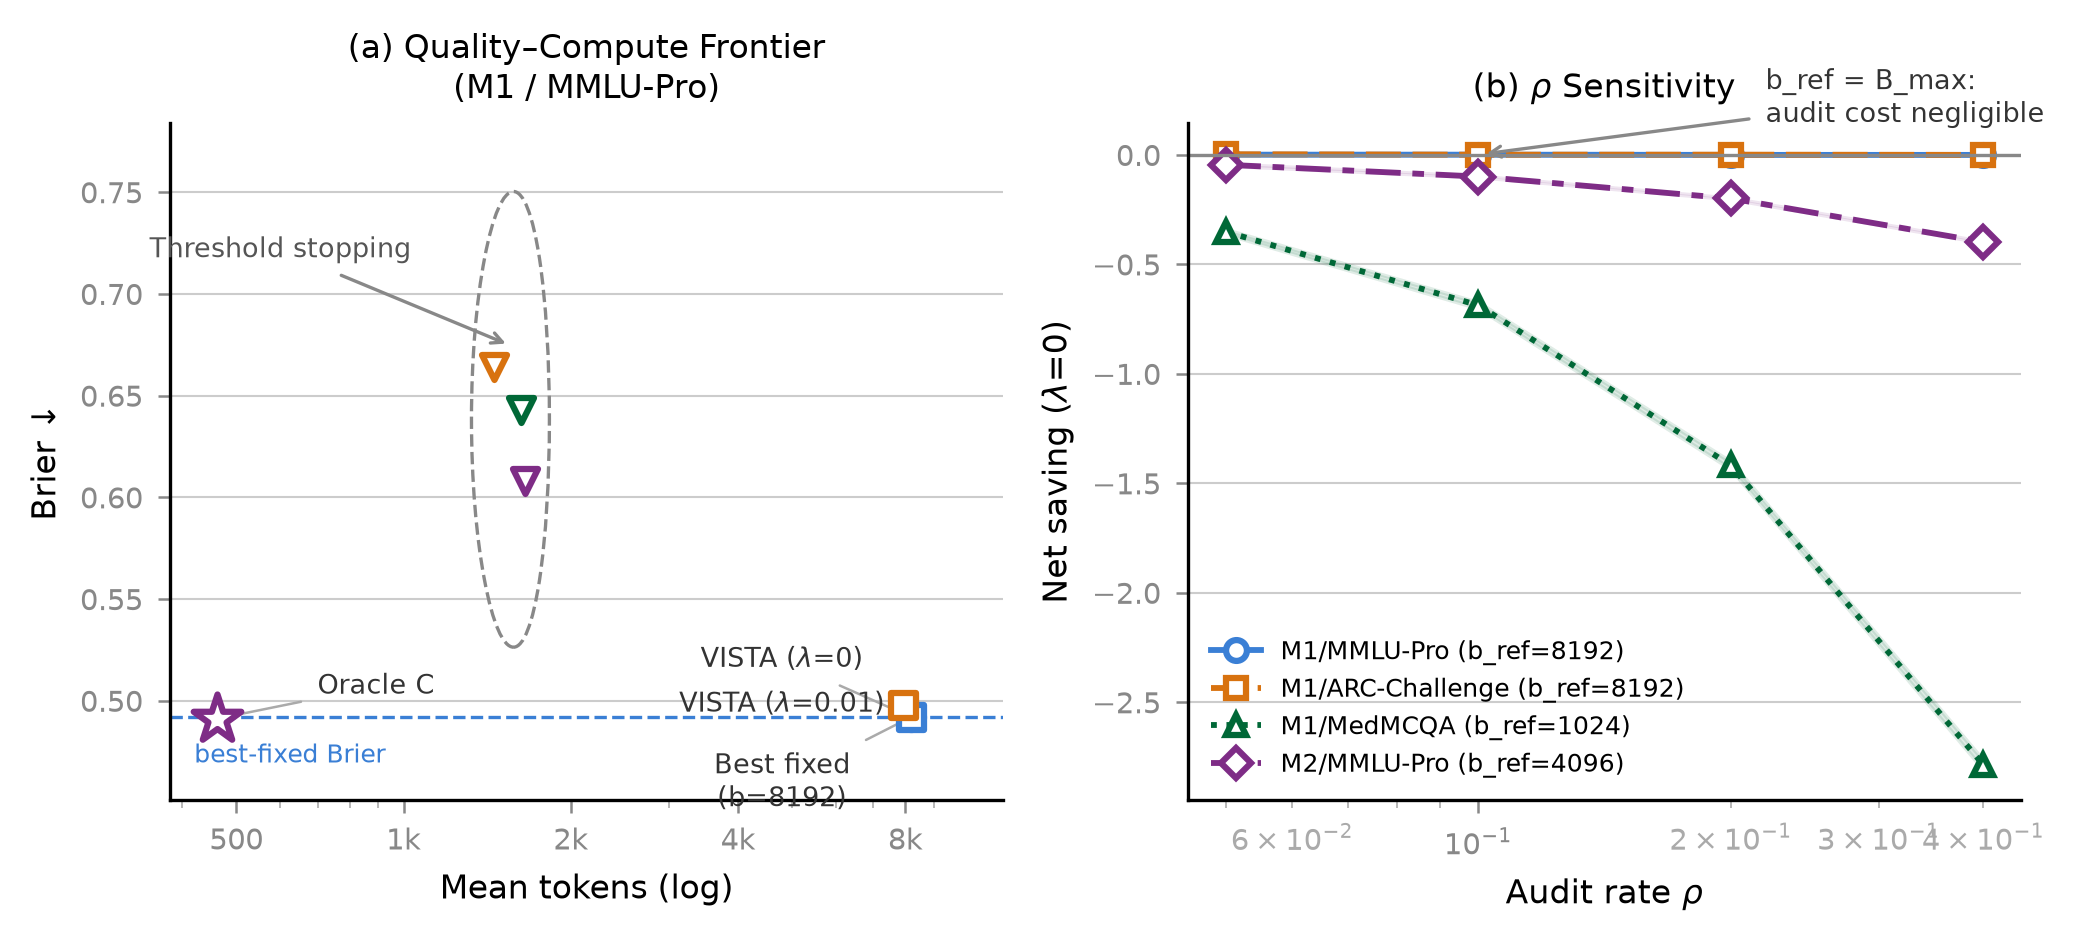
\includegraphics[width=\textwidth, height=0.55\textheight, keepaspectratio=true]{fig5.png}
\end{center}
\begingroup
\captionof{figure}{\textbf{(a) Quality--compute frontier for M1/DS1 (MMLU-Pro).}
    Each marker shows a deployed or oracle policy; $x$-axis is mean tokens
    per item (log scale), $y$-axis is summed Brier (\textbf{↓}).
    Threshold stopping policies (confidence, entropy, stability; triangle
    cluster) achieve large token reductions but degrade Brier by
    $+0.115$--$+0.172$ relative to the best-fixed baseline (dashed line).
    VISTA ($\lambda{=}0$) matches best-fixed quality at near-identical cost;
    VISTA ($\lambda{=}0.01$) gains $3.2\%$ token saving at the cost of
    $+0.006$ Brier.
    Oracle~C achieves near-identical Brier at $461$ mean tokens---the
    headroom available to future policy improvements.
    Data from Tables~\ref{tab:main} and~\ref{tab:gate0-oracle-c}.
    \textbf{(b) Audit-rate sensitivity ($\lambda{=}0$).}
    When $b_{\mathrm{ref}}{=}B_{\max}{=}8192$, audited items already run to
    the reference budget so audit overhead is negligible (lines near zero).
    When $b_{\mathrm{ref}}{<}B_{\max}$, each audited item pays the full
    $B_{\max}$ trajectory cost, making net saving strongly negative; these
    cells require $\lambda{>}0$ to be deployment-beneficial.
    Data from Table~\ref{tab:a07_rho_sensitivity}.}
\label{fig:frontier}
\endgroup
\vspace{\baselineskip}

\subsection{Robustness under Distribution Shift}
\label{sec:shift}

We simulate controlled distribution shift by splitting the deployment stream
at the dataset boundary: the first phase contains items from a source
dataset (phase~1), and the second phase transitions to a target dataset
(phase~2).
The prequential policy adapts its budget threshold online using arriving
feedback; the fixed policy freezes the threshold calibrated in phase~1.

The prequential policy outperforms fixed calibration in 3 of 8 scenarios
(mean advantage $+0.038$ Brier in those cases), and is marginally worse
in the remaining 5 (mean disadvantage $-0.007$ Brier).
The advantage is concentrated in domain-crossing transitions:
M1 benefits from within-medical shift (MedMCQA$\to$MedQA, $+0.037$), while
M2 benefits from general-to-medical shift
(MMLU-Pro$\to$MedMCQA $+0.039$ and MMLU-Pro$\to$MedQA\text{-USMLE} $+0.039$).
Difficulty-level shifts within the same domain (ARC-Challenge$\to$MMLU-Pro)
favour the fixed policy.
The prequential advantage requires a shift large enough to invalidate the
calibrated threshold; model-specific confidence dynamics modulate which
shifts cross that threshold.

\subsection{Measurement Validity}
\label{sec:validity}

Forced checkpoint evaluation appends a standardised answer-cue string and
reads next-token log-probabilities; in the diagnostic sample the target option
ranks first in $>98.4\%$ of cases, confirming stable elicitation.
Probability measurements are never pooled across GPU architectures: the two
RTX~3090 cards produce byte-identical logits (max $|\Delta\text{logprob}|=0.065$
at $b=8192$), while RTX~4090 and RTX~3090 differ non-negligibly (max $0.374$),
consistent with architecture-level kernel differences between sm\_89 and sm\_86;
each model$\times$dataset cell is therefore confined to a single architecture.
Stream-order permutations produce coefficient of variation $0.57\%$ on
MMLU-Pro, confirming negligible sensitivity to item ordering.
Forced and natural trajectory boundaries are distinguished throughout; natural
stopping is not equated to independently generated short-budget trajectories.

\FloatBarrier
%%%%%%%%%%%%%%%%%%%%%%%%%%%%%%%%%%%%%%%%%%%%%%%%%%%%%%%%%%%%%%%%%%%%%%%%%%%%%%
\section{Discussion}
%%%%%%%%%%%%%%%%%%%%%%%%%%%%%%%%%%%%%%%%%%%%%%%%%%%%%%%%%%%%%%%%%%%%%%%%%%%%%%

\paragraph{Finding 1: the marginal value of additional reasoning is not
universal.}
Budget-response curves differ qualitatively across tasks, models, objectives,
and budget intervals---in ways that cannot be resolved by choosing a larger
fixed budget.
On ARC-Challenge, 98\% of the potential Brier gain is captured in the first
budget step; on MedMCQA, continuing beyond $b=1024$ actively worsens Brier.
M2's Brier worsens at nearly every budget step on two of four datasets (MedMCQA and
MedQA-USMLE) while M1's improves; on MMLU-Pro, M2 Brier improves through
$b=4096$ and reverses slightly at the maximum budget.
Accuracy and proper-scoring-rule optima can differ by three budget levels on
the same dataset.
The consequence is that neither a fixed global budget nor a single heuristic
stopping rule can simultaneously optimise predictive quality, calibration, and
compute expenditure across the full range of deployment conditions.

\paragraph{Finding 2: trajectory signals are useful but not uniformly reliable
or transferable.}
Prefix signals---confidence, entropy, answer stability---predict the direction
of future improvement with AUC $0.65$--$0.81$ on MMLU-Pro (clearing the
pre-specified $\geq 0.60$ threshold on most edges), and answer stability
carries a non-trivial Spearman correlation ($\rho=0.31$) with improvement
magnitude.
These signals are genuinely informative as diagnostic tools.
However, two empirical failures limit their deployment utility.
First, confidence thresholds calibrated on one model fail on another on
domain-specific tasks (Brier degradation $+0.043$--$+0.073$ on transfer).
Second, applying a confidence gate directly at deployment increases Brier
above the best fixed budget in all eight cells ($+0.047$ to $+0.218$),
because signal direction is not a reliable proxy for outcome improvement at
the individual item level.
The signals therefore motivate the randomized-audit design rather than
replacing it: they establish that improvement \emph{potential} exists per
item, while the audit mechanism provides the outcome estimate needed to act
on it.

\paragraph{Finding 3: VISTA addresses the failures that signals cannot.}
Each VISTA component maps to one failure mode documented above.
IPW corrects the selection bias that emerges when only $0.1$--$18\%$ of items
naturally continue to the reference budget---bias that reverses policy
rankings in five of eight cells without correction.
Anytime-valid confidence sequences eliminate false-positive policy switching
($\mathrm{FPR}=0.000$ in all cells) while greedy monitoring reaches $58.5\%$
error rates on cells where multiple budget levels have near-equal risk.
Prequential calibration is beneficial under stationarity in 6 of 8 cells
(advantage up to $+0.047$ Brier) and provides the critical adaptation
mechanism under domain-crossing distribution shifts ($+0.037$--$+0.039$ Brier
in the strongest cases).

\paragraph{Cost of guarantees and negative results.}
Statistical guarantees have a non-trivial cost that must be stated clearly.
The CS procedure achieves FPR\,${=}\,0.000$ by construction, but this is achieved
by abstaining from switching when evidence is insufficient --- not by making correct
decisions.
At deployment horizon $n{=}200$ with $\rho{=}0.20$ (${\approx}40$ audits per cell;
full streams are $n{=}500$--$1000$), the CS procedure essentially never triggers
a switch at $\lambda{=}0$; its contribution at this horizon is safety (no false
switches) rather than adaptation (no switches at all).
The framework remains operationally useful at $\lambda{=}0.01$, where the
certifiable gap is wider and the CS bound can tighten: cells with $b_{\mathrm{ref}}{=}8192$
deliver 3--35\% net saving with Brier increases $\leq 0.012$.
Confidence-threshold stopping is a uniform negative result: it degrades Brier
in all eight cells ($+0.047$ to $+0.218$ versus best fixed budget).
Two cells are a genuine negative result: M2/MedMCQA and M2/MedQA have best-fixed
budget at $b{=}256$ (the grid minimum), leaving no adaptive headroom.
The framework correctly identifies and reports these no-opportunity regimes rather
than forcing an adaptation that does not exist.
Oracle~C (population-level) headroom remains $74$--$97\%$ in Gate-0-passing cells,
but the gap between Oracle~C saving and deployed saving ($0$--$35\%$) is the direct
cost of the statistical guarantee and limited stream length --- not a failure of the
approach.

\paragraph{Choosing $\lambda$ in practice.}
In practice, $\lambda$ should reflect the acceptable quality--compute exchange
rate at deployment.
The $\lambda{=}0.01$ results above offer a concrete reference point: this
setting yields $3$--$35\%$ net token savings at mean Brier increases of
$0.006$--$0.012$ across the three $b_{\mathrm{ref}}{=}b_{\max}$ cells
(M1/DS1: $3.2\%$, $+0.006$ Brier; M1/DS2: $34.5\%$, $+0.008$; M1/DS4:
$7.0\%$, $+0.012$; all with 95\% CIs from 200 permutations).
Practitioners with strict quality requirements should begin at $\lambda{=}0$---which
VISTA correctly renders quality-preserving---and increase $\lambda$
incrementally while monitoring realized Brier degradation against this
reference rate.

\paragraph{Limitations.}
Assumption~\ref{asm:feedback} restricts applicability to tasks with eventually
verifiable outcomes. The policy family is finite and pre-specified, so
guarantees concern only included candidates. Forced checkpoint evaluation is an
explicit intervention, not equivalent to independently generated short-budget
trajectories. Experiments are limited to 8B-parameter models on
single-workstation GPUs; whether patterns change at larger scales is an open
question. Randomized auditing incurs real compute costs that may conflict
with per-request latency constraints even when the long-run value is positive.
The asymptotic narrowing of the gap between Oracle~C and deployed VISTA
saving as $n_{\mathrm{aud}}\!\to\!\infty$ is not empirically verifiable at
the dataset scales tested here ($n\leq 1000$): per-item combined-loss
signal-to-noise ratios are too low for consistent CS certification in this
regime, and extending empirically requires substantially larger corpora or
bootstrap resampling outside the anytime-valid guarantee.

%%%%%%%%%%%%%%%%%%%%%%%%%%%%%%%%%%%%%%%%%%%%%%%%%%%%%%%%%%%%%%%%%%%%%%%%%%%%%%
\section{Conclusion}
%%%%%%%%%%%%%%%%%%%%%%%%%%%%%%%%%%%%%%%%%%%%%%%%%%%%%%%%%%%%%%%%%%%%%%%%%%%%%%

We study test-time reasoning-budget selection in a deployment regime with no
held-out calibration set but delayed verifiable feedback. Three interlocking
obstacles---correctness non-identifiability, the missing continuation
counterfactual, and the absence of a calibration split---motivate the
\emph{continuation value} as the decision target and the VISTA
prequential framework as the evaluation procedure. VISTA combines randomized
full-trajectory audits, candidate policy reconstruction, delayed labels, and
anytime-valid confidence sequences without reserving a separate split or
updating model parameters.

A systematic budget audit across eight cells (two models, four datasets)
confirms that the marginal value of additional reasoning is strongly
task- and budget-dependent.
Accuracy gains range from near-linear (MMLU-Pro: 47.7\% $\to$ 73.8\%) to
early-saturating (ARC-Challenge: 92.0\% $\to$ 95.8\%), while proper-scoring-rule
and NLL optima can diverge from the accuracy optimum within the same dataset.
On MMLU-Pro the hindsight oracle (Oracle~A) reduces mean Brier by 30.1\%
relative to the best fixed budget; 76.1\% of items meet a per-item quality
threshold at a budget below the global maximum (Oracle~B).
The constrained matched-mean-quality oracle (Oracle~C) passes Gate~0 in
six of eight cells, with savings from 74\% to 97\% relative to the best fixed
budget; the two failing cells (M2 MedMCQA and MedQA-USMLE) have Brier
worsening at all budgets above the minimum, leaving no adaptive headroom
under a mean-Brier constraint.

Component ablations confirm that each element of VISTA addresses a distinct
failure mode. Naive policy risk estimation carries selection bias that reverses
policy rankings in 5 of 8 cells; IPW corrects this with mean bias $\leq 0.033$.
Anytime-valid confidence sequences eliminate false-positive policy switching
(FPR\,${=}\,0.000$ across all cells) at the cost of conservative time-to-decide.
Confidence thresholds do not transfer reliably across model families on
domain-specific tasks, motivating per-model prequential calibration.
Full end-to-end VISTA evaluation across all eight cells completes the picture:
at $\lambda{=}0$, the procedure is quality-preserving (CS correctly declines to
certify cheaper policies on 200-item streams); at $\lambda{=}0.01$,
deployable net savings of $3$--$35\%$ with Brier increases $\leq 0.012$ are
achievable in cells where calibration saturates early.
The two no-opportunity cells (Brier worsens above minimum budget) are a genuine
negative result that the framework correctly identifies rather than masks.

\section*{Data and Code Availability}
Code and cached checkpoint tables (all per-item, per-budget predictive
distributions) will be released in a public repository upon acceptance under
an open-source license (URL and license identifier to be confirmed at
acceptance).
The online policy-selection procedure is fully replayable from these tables
without GPU inference.

\section*{Acknowledgements}
Experiments were conducted on a personal workstation equipped with one
NVIDIA RTX~4090 and two RTX~3090 GPUs; no external compute grant was
used.
The authors gratefully acknowledge the Qwen team at Alibaba Cloud for
releasing Qwen3-8B and the DeepSeek team for releasing
DeepSeek-R1-Distill-Llama-8B under open-source licenses, and the curators
of MMLU-Pro~\cite{wang2024mmlu}, ARC-Challenge~\cite{clark2018arc},
MedMCQA~\cite{pal2022medmcqa}, and MedQA-USMLE~\cite{jin2021medqa}
for making their benchmarks publicly available.
All experiments use publicly available model weights and benchmark data;
no human subjects were involved.

\section*{Funding}
This research did not receive any specific grant from funding agencies in
the public, commercial, or not-for-profit sectors.

\section*{CRediT authorship contribution statement}
\textbf{Jun-young Kong:} Conceptualization, Methodology, Software, Formal
analysis, Investigation, Data curation, Visualization, Writing~-- original draft.
\textbf{Young-guk Ha:} Supervision, Writing~-- review \& editing.

\FloatBarrier
%%%%%%%%%%%%%%%%%%%%%%%%%%%%%%%%%%%%%%%%%%%%%%%%%%%%%%%%%%%%%%%%%%%%%%%%%%%%%%
\bibliographystyle{elsarticle-num}
\bibliography{mvtcs}
%%%%%%%%%%%%%%%%%%%%%%%%%%%%%%%%%%%%%%%%%%%%%%%%%%%%%%%%%%%%%%%%%%%%%%%%%%%%%%


%%%%%%%%%%%%%%%%%%%%%%%%%%%%%%%%%%%%%%%%%%%%%%%%%%%%%%%%%%%%%%%%%%%%%%%%%%%%%%
\appendix
\section{Component Ablation Supplementary Tables}
\label{app:ablation_tables}
%%%%%%%%%%%%%%%%%%%%%%%%%%%%%%%%%%%%%%%%%%%%%%%%%%%%%%%%%%%%%%%%%%%%%%%%%%%%%%

Table~\ref{tab:a01_ipw_naive} reports per-cell IPW versus naive estimation
bias and wrong-best-budget selection rates at $\rho=0.20$.
Table~\ref{tab:a03_cs_greedy} compares anytime-valid confidence-sequence
monitoring with greedy monitoring.
Table~\ref{tab:a07_rho_sensitivity} reports audit-rate sensitivity across
representative cells.
Tables~\ref{tab:a20_component_removal} and~\ref{tab:a20b_component_lambda001}
present the deployed-policy decomposition for M1/MMLU-Pro at $\lambda=0$
and $\lambda=0.01$ respectively.

% ===========================================================================
% Table 9 — A01 IPW vs. naive
% ===========================================================================

\Needspace{0.37\textheight}
\par\medskip

\begin{center}
\begin{minipage}{0.92\textwidth}
\centering

\captionsetup{
  font=small,
  skip=5pt,
  justification=justified,
  singlelinecheck=false
}

\small
\setlength{\tabcolsep}{5.2pt}
\renewcommand{\arraystretch}{0.98}

\begin{tabular}{@{}lrrrrr@{}}
\toprule
Cell &
$f_{\mathrm{nat}}$ &
Naive bias &
IPW bias &
$\epsilon_{\mathrm{naive}}$ &
$\epsilon_{\mathrm{IPW}}$ \\
\midrule
m1\_ds1 & 0.122 & 0.07079 & 0.02447 & 0.000 & 0.230 \\
m1\_ds2 & 0.001 & 0.23535 & 0.01031 & 1.000 & 0.630 \\
m1\_ds3 & 0.018 & 0.34441 & 0.02634 & 1.000 & 0.555 \\
m1\_ds4 & 0.028 & 0.28715 & 0.03207 & 1.000 & 0.455 \\
m2\_ds1 & 0.180 & 0.04562 & 0.02092 & 1.000 & 0.525 \\
m2\_ds2 & 0.007 & 0.13616 & 0.01176 & 0.000 & 0.615 \\
m2\_ds3 & 0.022 & 0.23482 & 0.02035 & 1.000 & 0.185 \\
m2\_ds4 & 0.052 & 0.10917 & 0.02986 & 0.000 & 0.525 \\
\bottomrule
\end{tabular}

\captionof{table}{
IPW vs.\ naive risk estimation at $\rho=0.20$ across all experimental cells.
$f_{\mathrm{nat}}$ denotes the fraction of items that naturally continue to
the reference budget (4096 tokens), and $\epsilon$ denotes the
wrong-best-budget selection rate over 200 stream-order permutations.
}
\label{tab:a01_ipw_naive}

\end{minipage}
\end{center}

\vspace{0.55\baselineskip}


% ===========================================================================
% Table 10 — A03 CS vs. greedy monitoring
% ===========================================================================

\Needspace{0.34\textheight}
\par\medskip

\begin{center}
\begin{minipage}{0.88\textwidth}
\centering

\captionsetup{
  font=small,
  skip=5pt,
  justification=justified,
  singlelinecheck=false
}

\small
\setlength{\tabcolsep}{5.5pt}
\renewcommand{\arraystretch}{0.98}

\begin{tabular}{@{}llrrr@{}}
\toprule
Cell &
Dataset &
CS FPR $\downarrow$ &
Greedy FPR $\downarrow$ &
Oracle $b^\star$ \\
\midrule
m1\_ds1 & MMLU-Pro       & 0.0000 & 0.0700 & 8192 \\
m1\_ds2 & ARC-Challenge  & 0.0000 & 0.4800 & 8192 \\
m1\_ds3 & MedMCQA        & 0.0000 & 0.4000 & 1024 \\
m1\_ds4 & MedQA-USMLE    & 0.0000 & 0.1400 & 8192 \\
m2\_ds1 & MMLU-Pro       & 0.0000 & 0.5850 & 4096 \\
m2\_ds2 & ARC-Challenge  & 0.0000 & 0.2500 & 2048 \\
m2\_ds3 & MedMCQA        & 0.0000 & 0.0000 & 256 \\
m2\_ds4 & MedQA-USMLE    & 0.0000 & 0.0000 & 256 \\
\bottomrule
\end{tabular}

\captionof{table}{
Anytime-valid confidence sequences (CS) versus greedy monitoring:
false-positive policy-switch rates at $\rho=0.20$ and $\alpha=0.05$
over 200 stream-order permutations.
}
\label{tab:a03_cs_greedy}

\end{minipage}
\end{center}

\vspace{0.65\baselineskip}


% ===========================================================================
% Table 11 — A07 audit-rate sensitivity
% ===========================================================================

\Needspace{0.58\textheight}
\par\medskip

\begin{center}
\begin{minipage}{0.94\textwidth}
\centering

\captionsetup{
  font=footnotesize,
  skip=5pt,
  justification=justified,
  singlelinecheck=false
}

\footnotesize
\setlength{\tabcolsep}{4.6pt}
\renewcommand{\arraystretch}{0.96}

\begin{tabular}{@{}llrrrr@{}}
\toprule
Cell &
$\rho$ &
Audit tokens &
Net saving &
95\% CI &
Brier \\
\midrule

\multirow{4}{*}{M1/MMLU-Pro}
 & 0.05 & 0.4    & $+0.001$ & $[+0.000,+0.002]$ & 0.4919 \\
 & 0.10 & 0.6    & $+0.001$ & $[+0.000,+0.001]$ & 0.4918 \\
 & 0.20 & 0.4    & $+0.000$ & $[-0.000,+0.000]$ & 0.4918 \\
 & 0.40 & 0.5    & $+0.000$ & $[+0.000,+0.000]$ & 0.4918 \\

\midrule

\multirow{4}{*}{M1/ARC-Challenge}
 & 0.05 & 1.0    & $+0.003$ & $[+0.001,+0.005]$ & 0.0839 \\
 & 0.10 & 1.1    & $+0.001$ & $[+0.001,+0.002]$ & 0.0838 \\
 & 0.20 & 1.1    & $+0.001$ & $[+0.000,+0.001]$ & 0.0838 \\
 & 0.40 & 1.1    & $+0.000$ & $[+0.000,+0.000]$ & 0.0837 \\

\midrule

\multirow{4}{*}{M1/MedMCQA}
 & 0.05 & 360.1  & $-0.351$ & $[-0.361,-0.341]$ & 0.6276 \\
 & 0.10 & 704.0  & $-0.687$ & $[-0.700,-0.674]$ & 0.6275 \\
 & 0.20 & 1452.3 & $-1.418$ & $[-1.434,-1.402]$ & 0.6275 \\
 & 0.40 & 2853.1 & $-2.786$ & $[-2.807,-2.766]$ & 0.6275 \\

\midrule

\multirow{4}{*}{M2/MMLU-Pro}
 & 0.05 & 205.1  & $-0.045$ & $[-0.048,-0.041]$ & 0.8788 \\
 & 0.10 & 407.8  & $-0.099$ & $[-0.100,-0.097]$ & 0.8783 \\
 & 0.20 & 820.6  & $-0.199$ & $[-0.201,-0.197]$ & 0.8783 \\
 & 0.40 & 1632.5 & $-0.398$ & $[-0.400,-0.396]$ & 0.8783 \\

\bottomrule
\end{tabular}

\captionof{table}{
Audit-rate sensitivity ($\lambda=0$): net saving and Brier as a function of
$\rho$ across representative cells.
When $b_{\mathrm{ref}}=b_{\max}=8192$, audit overhead is negligible because
audited items already run to the reference budget.
When $b_{\mathrm{ref}}<b_{\max}$, full-trajectory auditing incurs additional
compute that grows with $\rho$, illustrating the explicit cost of statistical
exploration.
}
\label{tab:a07_rho_sensitivity}

\end{minipage}
\end{center}

\vspace{0.65\baselineskip}


% ===========================================================================
% Table 12 — A10 component-removal analysis
% ===========================================================================

\Needspace{0.43\textheight}
\par\medskip

\begin{center}
\begin{minipage}{0.92\textwidth}
\centering

\captionsetup{
  font=small,
  skip=5pt,
  justification=justified,
  singlelinecheck=false
}

\small
\setlength{\tabcolsep}{5.3pt}
\renewcommand{\arraystretch}{0.98}

\begin{tabular}{@{}lrrrr@{}}
\toprule
Variant &
Brier $\downarrow$ &
Tokens &
Net saving &
Regret vs.\ oracle \\
\midrule

\multicolumn{5}{@{}l}{
\textit{Item-level adaptation}
} \\

Confidence-threshold policy ($\tau_c=0.85$)
 & 0.6831 & 1273 & $+0.845$ & 0.339 \\

VISTA ($\lambda=0$) --- no switch certified
 & 0.4917 & 8192 & 0.000 & 0.148 \\

\midrule

\multicolumn{5}{@{}l}{
\textit{Monitoring components ($\lambda{=}0$, $\rho{=}0.20$, 200 permutations)}
} \\

$-$ Audit/IPW
 & 0.4917 & 8192 & $0.000$ & 0.148 \\

$-$ CS (greedy switch)
 & 0.522  & 5838 & $+0.288$ & 0.179 \\

\bottomrule
\end{tabular}

\captionof{table}{
Deployed-policy decomposition at $\lambda=0$ (M1/MMLU-Pro,
$\rho=0.20$, $n=1000$, 200 stream permutations).
\textit{Item-level adaptation:} the confidence-threshold stopping policy
and the full-budget Fixed@8192 baseline span the practical range.
\textit{Monitoring components:} removing IPW leaves the outcome unchanged
because at $\lambda=0$ the cost-adjusted loss of all cheaper policies
exceeds Fixed@8192's Brier regardless of bias correction --- the CS
correctly certifies no switch either way.
Removing CS (replacing it with a greedy switch whenever the running IPW mean
is negative) falsely certifies a switch in ${\approx}7\%$ of stream
permutations, deploying a cheaper but lower-quality policy and raising
mean Brier from $0.492$ to $0.522$ ($+3.0$ pp).
The bias-reduction contribution of IPW and the false-positive-rate control
of CS are therefore measured in dedicated ablations
(Tables~\ref{tab:a01_ipw_naive} and~\ref{tab:a03_cs_greedy}) rather than
through deployment metrics at $\lambda=0$.
Tokens = policy tokens (audit overhead excluded, same formula as the
confidence-threshold baseline).
Regret = deployed Brier $-$ per-item oracle Brier ($0.3437$).
}
\label{tab:a20_component_removal}

\end{minipage}
\end{center}

\vspace{0.65\baselineskip}

% ===========================================================================
% Table 12b — Component decomposition at lambda=0.01
% ===========================================================================

\Needspace{0.42\textheight}
\par\medskip

\begin{center}
\begin{minipage}{0.92\textwidth}
\centering

\captionsetup{
  font=small,
  skip=5pt,
  justification=justified,
  singlelinecheck=false
}

\small
\setlength{\tabcolsep}{5.3pt}
\renewcommand{\arraystretch}{0.98}

\begin{tabular}{@{}lrrrr@{}}
\toprule
Variant &
Brier $\downarrow$ &
Tokens &
Net saving &
Regret vs.\ oracle \\
\midrule

\multicolumn{5}{@{}l}{
\textit{$\lambda{=}0.01$, $\rho{=}0.20$, 200 stream permutations (M1/MMLU-Pro)}
} \\

VISTA ($\lambda=0.01$, full)
 & 0.498 & 7871 & $+0.039$ & 0.154 \\

$-$ Audit/IPW
 & 0.498 & 7871 & $+0.039$ & 0.154 \\

$-$ CS (greedy switch)
 & 0.529 & 5386 & $+0.343$ & 0.185 \\

\bottomrule
\end{tabular}

\captionof{table}{
Component decomposition at $\lambda=0.01$ (M1/MMLU-Pro,
$\rho=0.20$, $n=1000$, 200 stream permutations).
At $\lambda=0.01$ the cost penalty is small enough that the CS rarely
certifies a switch ($<5\%$ of streams), so removing IPW again leaves
outcomes unchanged: the bias in naive estimates is insufficient to alter
the certified decision.
Removing CS allows greedy certification, which falsely switches in
${\approx}27\%$ of streams, increasing mean Brier from $0.498$ to $0.529$
($+3.1$ pp) while spuriously appearing to save $34\%$ of tokens.
The pattern confirms that the CS is the operative safety mechanism across
both cost-penalty settings: IPW primarily reduces estimation bias for the
rare certified-switch events recorded in Table~\ref{tab:a01_ipw_naive}, while
CS prevents the false-positive switches visible in Table~\ref{tab:a03_cs_greedy}.
Same column definitions as Table~\ref{tab:a20_component_removal}.
Table~\ref{tab:main} reports 7931 tokens for the same policy including the $\rho{=}0.20$ audit overhead; tokens here exclude it, following Table~\ref{tab:a20_component_removal}.
}
\label{tab:a20b_component_lambda001}

\end{minipage}
\end{center}

\vspace{0.4\baselineskip}

%%%%%%%%%%%%%%%%%%%%%%%%%%%%%%%%%%%%%%%%%%%%%%%%%%%%%%%%%%%%%%%%%%%%%%%%%%%%%%
\end{document}
%%%%%%%%%%%%%%%%%%%%%%%%%%%%%%%%%%%%%%%%%%%%%%%%%%%%%%%%%%%%%%%%%%%%%%%%%%%%%%


